% Chapter 1

\chapter{Infrastructure Management System} % Write in your own chapter title
\label{Chapter2}
\lhead{Chapter 2. \emph{Infrastructure Management System}} % Write in your own chapter title to set the page header
%%%
This chapter reviews the profound research works on the field of infrastructure asset management, which was developed by asset management team at Kyoto University lead by Professor Kiyoshi Kobayashi. Many of prominent scholars had involved in developing one the most advance stochastic model on hazard analysis, which becomes a solid base for the latter investigation on this field. Main references are the paper on multi-stage exponential hazard model \cite{kobayashitsuda} and paper on measuring deterioration risk of infrastructure \cite{aokib}.
\section{General introduction}
\label{21}
In recent years, infrastructure management study has attracted a great attention, especially in developed countries. After the fast growing economic period in $20^{th}$ century, a great number of major construction works such as: pavement, bridge, tunnel, dam, airport, etc are projected to be in the status with fault performances and obsolescence. The downturn in the performance and functionality of infrastructure system, as a whole, imposes heavy burdens on various aspects of the socio-economic. In response, there is no way but having to wisely mobilize and allocate proper resources into right places, at the right time, to uphold the smooth service levels. Technically, this task turns to be the mission of ``how to establish a systemic asset management'', which is realized heavily depending on hazard models and life cycle cost evaluation techniques.

Asking for hazard models, there are two classified modeling approaches, deterministic and stochastic. Deterministic model simulates the degradation of infrastructure structure, component by analyzing physical functionality, which can be described as a deterministic function of several prominent characteristic variables. This approach often requires experiments in laboratory. On the other hand, stochastic modeling requires a huge monitoring data, which is often technical and financial difficulty.

Under a microscopic view, deterministic approach is relevant to be applicable for a small range of infrastructure, where experimental works can be proposed. However, in fact, most of infrastructure asset is in a vast scale and under a dynamic impact from environmental conditions. It is therefore, for macroscopic standpoint, stochastic modeling would become a much prefer alternative to deterministic one.

Whatever deterministic or stochastic approach is employed, the task for management remains unchanged. It is, a selection of a good model, which can simulate the actual behavior of system, minimize the uncertainty and can propose a list of proactive activities (maintenance, repair, renovation) in the most optimized technical and economical expectations. However, selection of the best suitable model is not an easy assignment under a dynamic system, particularly in macroscopic view (network level), where multi-objectives for management are often encountered.

%A network of integrated infrastructures adds another considerable task since each sub-system exerts its deterioration differently from others, and thus further require a distinguish deterioration model.
%
There are many problems when dealing with network level of infrastructure management. Among them, the problem due in the recording from monitoring and inspection is an outstanding. Truly, it can be because of the system complexity, where various performance indicators are obligated to be measured. However, we often fail to do so. 
%Further to network level, which is the main targeted system of this research, it is understood that high uncertainty and complexity exist in management of the entire infrastructure system. For example, in pavement management system (PMS) of a city, deterioration of road sections is influenced by various factor such as: traffic volume, bearing capacity of foundation, thickness of structures. The values of those factors keep changing along with time, and thus require an accurate monitoring. However, monitoring or inspection might not be carried out according to expectation and guidelines. As the sequent, mistakes in reporting for repair actions and budget allocation might spoil the accuracy of decisions. 
This appealing problem in management of network level has generated a voluminous literatures and effort in establishing various systemic asset management programs through development of hazard and cost evaluation models.

In stochastic estimation approach, hazard model is formulated based on probabilistic assumption of transition of condition states, which reflect the healthy status of the system. Condition states are actually recorded as historical data through monitoring and inspection over periods of time \footnote{year is often used for infrastructure monitoring and inspection}. In many cases, small sampling populations and measurement errors are turned out, and consequently cause bias in estimation results \cite{kobahidden}. Therefore, it is necessary at the outset of this study to emphasize the development and estimation approach of deterioration hazard models, which are formulated based on observation of inspection data by means of probability and statistical contexts.

The following section gives background literatures on infrastructure asset management, where emphases are on quality assurance through management cycle, recent development of stochastic reliability using Markov chain model and the importance of monitoring. Section \ref{23} presents assumption and formulation of hazard models based on Markov chain theory. A brief discussion on estimation approach for respective hazard model is presented in section \ref{24}. The subsequence section \ref{25} further discusses the application of Bayesian estimation in a new type of hazard model dealing with measurement errors. The last part of this chapter highlights estimation results of an empirical study conducted on the database of tunnel lighting utility.
%%
\section{Background}
\label{22}
\subsection{Overview of Infrastructure Management System}
\label{221}
At first, a brief introduction to the objectives, missions, and functions of the entire infrastructure asset management would be necessary before entering to discover the relationship between statistical model and monitoring. The management structure is hierarchical management system encompassing of three distinguish managerial levels as displayed in Figure. \ref{fig21}. The first top strategic level deals with management mission for long-term implementation. The second strategic management level focuses on the plans and related activities for medium-term implementation. Whilst, the bottom level in the hierarchical management system concerns with a specific maintenance and repair works. 

Each level of management has its own missions and objectives as well as requires a specific analytical methodology. However, the three levels are integrated into a single functional entity for entire network structure.
%
\begin{figure}[t]
\begin{center}
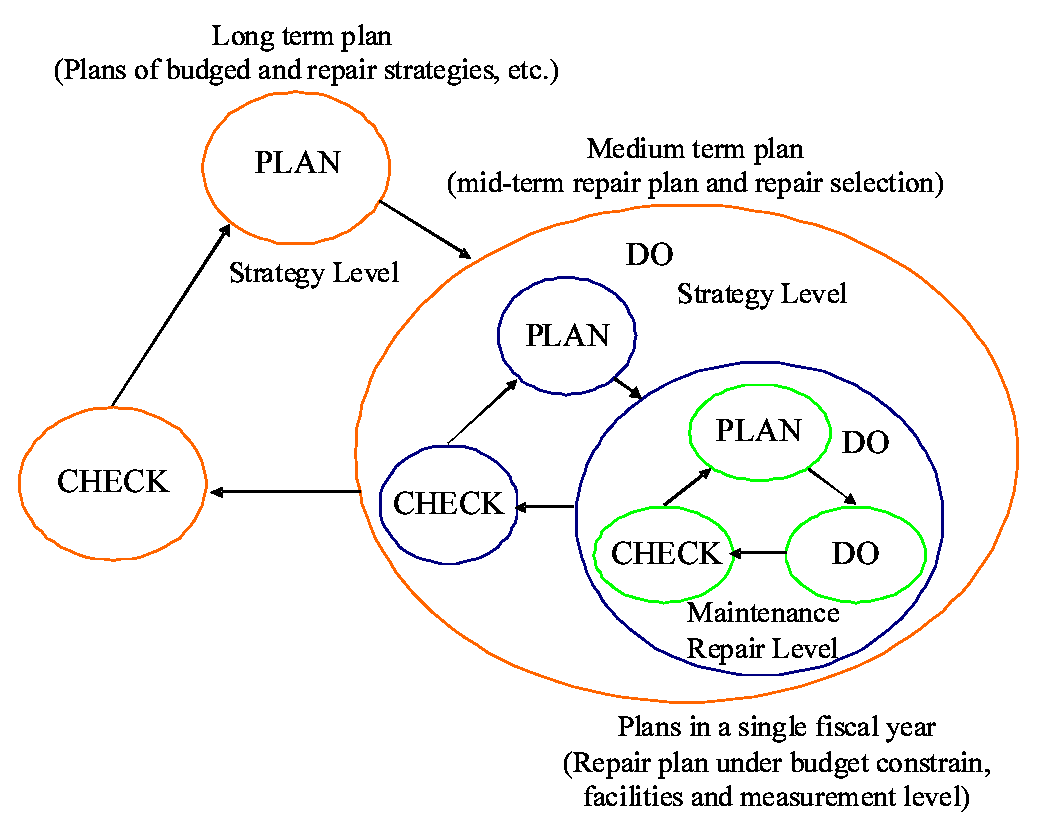
\includegraphics[scale=0.5]{fig21} 
\end{center}
\caption{Hierarchical Management Cycle.}
\label{fig21} 
\end{figure}

Management at top strategic level is understood as management of infrastructure network. The entire network is an integration or link of many infrastructure facilities. The objectives of management at network level are to define the service level for each group of infrastructure facility. This is an essential task in order to ensure the satisfaction and safety demanding from society. If the service level falls into poor status, as a sequent, various negative impacts will occurred. For example, bearing capacity of bridge concrete slab must always be in the range of acceptance \footnote{The bearing capacity of slab must always-above safety level, which is designated in structural analysis}. Otherwise, a collapse would happen that may not only cause economical loss but also claims the loss of life in some extend.

Further to long-term plan, one of the important assignment is ``How to evaluate and allocate a proper budget quota for each type or group of infrastructure''. In fact, budget allocation must be rigorously estimated by means of life cycle cost evaluation technique, which, in return, depending largely on the selection of the target service level, maintenance, and repair strategy. In practice, it is often the case that a set of the best maintenance and repair strategies are recommended for long-term management. The integration of hazard model and life cycle cost analysis becomes a vital tool to establish a state of control, a set of the best maintenance and repairs, which turns out to be the inputs or indicators for planning of the later phases.

Asking for middle-term plan, under the circumstance that a clear guidelines and outputs of long-term plan already established, the objective is to setting up a execution plan, which lists up the maintenance and repair activities on respective infrastructure facilities according to the priorities and the exposing risks. The top listed activities are expected to execute on the infrastructures, which expose to high-risk levels, having fast deteriorations and playing important service roles. In order to propose an appropriate list of actions, a sound monitoring system and measurement shall be engaged.

Regarding the management and repair level, which is often carried out within a fiscal year, budget allocation becomes a critical factor. Given the amount of fixed money from government and the priority list of action decided for middle-term plan, a detailed work break down structure for actual execution will be issued. In essence, the specific maintenance and repair will be scheduled according to its priority level and in connection with operation time of facilities. It is important at this stage to thoughtfully examine and record the actual performance of facilities and further document its updated status into inventory system.

As can be further discussed from the Figure \ref{fig21}, at all three levels of management, quality of work must be assured. Therefore, the Deming cycle \cite{deming} (PLAN-DO-CHECK) plays a center role. Any negligent performance may consequently lead to failure of management objectives at all levels. At first, a regular CHECK by mean of monitoring and inspection shall be well established. Secondly, a feasible PLAN with list of actions must be defined. Finally, implementing DO according to specification and guidelines \footnote{Deming cycle is widely applied in quality management, especially in business and operation of industrial factories. The center role of the cycle is toward continuous improvement of quality. A widely used abbreviation of the cycle is PDCA, meaning Plan, Do, Check, and Acts}.
%%%%%%%%%%%%%%%%%
\subsection{The Role of Hazard Model}
\label{222}
As previously explained, one of the important role in the control process for maintenance of infrastructure facility is to preserve facilities in smooth service standing. As the deterioration progresses by time, it turns out to be the task for maintenance and renovation of facilities, to keep the performance indicators in acceptable ranges. In this situation, the state of control and deterioration influencing factors must be accurately measured. By inspection and monitoring, we are able to keep an eye on the actual performance indicators. However, management and maintenance are also further extended to cover the future allocation of resources. This is therefore; hazard should be in place for predicting the progress of degradation, and for evaluating prominent environment factors contributing to the process. In essence, it is true to state that hazard model is the core of any infrastructure management program. Up to present, abundant of researches have been extensively documented with increasing emphasis on the dynamic deterioration mechanism \cite{kagi,kobami,tutu2,ono,qi,saeki}.

With respect to strategic level of management, the role of hazard model is to assist the selection for the state of control, the best guidelines for construction, maintenance, and repair, etc through the life cycle cost analysis. However, the difficulties are often encountered due to the demand in smoothly controlling and managing at the same time for hundreds or thousands of infrastructure facilities. Simply because, each infrastructure facility exerts to different deterioration behaviors due to variation of operation time, environment conditions and working loads. This task can only be successfully done through a hazard model, which considers all that factors for defining an average trend of deterioration for entire system. In fact, this approach is statistical dynamic oriented process that its accuracy largely relies on the accurate level in inspection and monitoring.

%Statistical hazard model toward dynamic deterioration mechanism with its advantages thus becomes the best method to address the deterioration problem in infrastructure asset management study and practice both at project and network point of views. Efforts in estimating average deterioration process of large number of infrastructure facilities have been carried out by using the information data from inspections \cite{kaito2}. 
%
To date, most of the hazard models have employed probabilistic and statistical approach, whereby, the state of control for infrastructure component is designated in discrete numbering range. The deterioration of infrastructure facility is simulated as transition pattern from one condition state to another condition state. However, the deterioration process bears its own uncertainty due to various endogenous and exogenous factors. To address this matter, it has been realized in recent years that the Markov chain model can be used to define the transition probability among the condition states. Interestingly, Markov chain model has been proved as the best applicable model in the sense of statistic and probability \cite{Takeyama,kenichi,Noriyuki}.

Further to Markov chain hazard model, much of the elaboration in estimating transition probability with inspection data is numerically estimated via maximum likelihood estimation technique. However, the challenges and difficulties somewhat belongs to how fit the assumption and presumption of model to be, and with respect to each type of infrastructure facility. Example of effort can be referred to Weibull hazard model for prediction the start of crack on pavement surface \cite{shin}, which typically discussed the issues of estimation under the missing of sufficient inspection data. The appealing challenge of presumption, on the other hand, opens the room for a large distribution of ongoing and future researches.

Keeping abreast of development trend in asset management, which tends to cope with the dynamic complexity of deterioration process and the trend of management, this research continues developing hazard model into several ankles, from a model which can apply generally on different type of infrastructure, to a specific model applied on a distinguish system. Special attention would be on presumption of parameters, embedded variables in hazard function and estimation approaches. In addition, empirical works shall be well addressed to link the theoretical part with practical implementation.
%%%%%%%%%%%%%%%%%%%%%
%\subsection{Future Perspectives of Asset Management}
%\label{223}
%Future fashion of infrastructure asset management system, as a matter of fact, depends much on the roles of the the system itself. In line with the overview of infrastructure asset management system, which already mentioned earlier with three levels of management, it is realized that the primary function of infrastructure asset management is resource management at all levels. Thus, if putting the future perspectives of infrastructure asset management on agenda, obvious to say, it is about the trails of how resources are going to be allocated. Thus, let us describe four trails of postulates which will justify the outlook of future asset management \footnote{The four trails are modified from \citet{bevpeter}}. Figure \ref{fig22} gives an idea of how the four trails link to corresponding aspects of management. 
%
%\begin{figure}[t]
%\begin{center}
%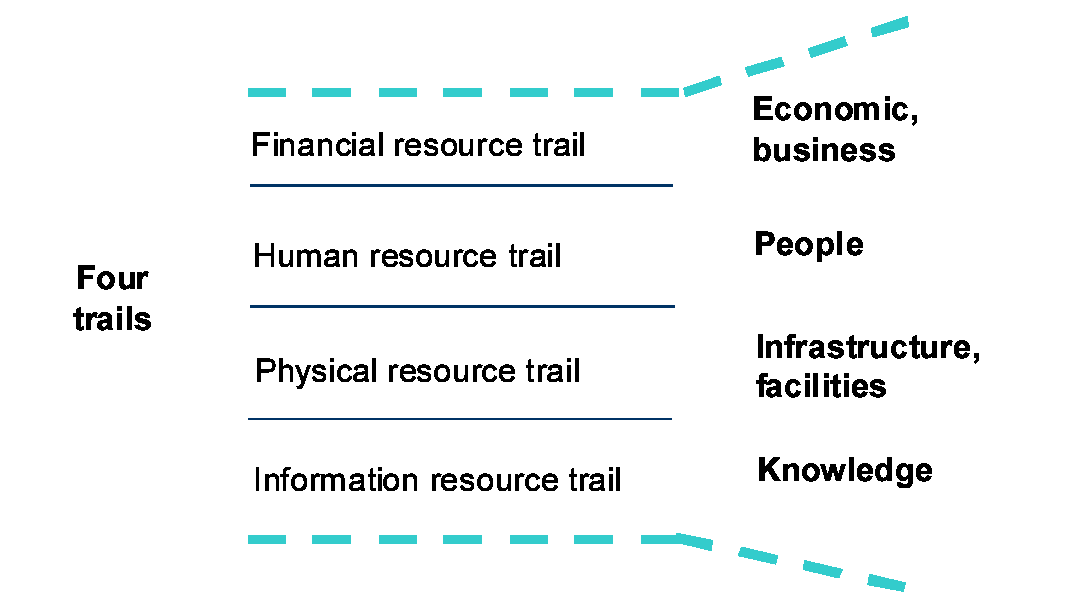
\includegraphics[scale=0.5]{fig22} 
%\end{center}
%\caption{Four generic trails of asset management to the future}
%\label{fig22} 
%\end{figure}
%
%\begin{itemize}
%\item{The financial trail will be the first to be discussed mainly due to the reasons that budget allocation for future construction work, which asset management accounts for a large share, is always of necessity. The question of how much, to where and when for maintenance and repair works should be tackle so as satisfying the equilibrium of resources in a long run. In addition, evaluation of infrastructure facilities in the view point of economic and finance eventually assist the formulation of best practices, best state of control, best maintenance and repair strategies for respective group of infrastructure. As the sequent, releasing heavy burdens of cost for society. The financial trails can also be further learned from the way that capital is mobilized among various stakeholders in society. For example, the participation of private section may change the traditional management fashion of public asset management in another form, which needs a carefully investigation so as service role of infrastructure can be sustained. A good solution in term of budget planning will hopefully enable future growth in sustainability.}
%
%\item{The human resource trail, as the second trail to be explored, could become the most revolutionary route to the future. A strong tendency has been realized that the working condition is projected to move in a dynamic and flexible form in the future with aids of advance technology, especially the ICT technology \cite{bevpeter}. Thus, the human resource deployment in the field of asset management should be well responded to ``place-flexibility'' and ``time flexibility'', probably towards a form of logistics management. In another word, the human resource logistic will need to become accountable for operational capacity, contingency provision, operational performance and operational effectiveness.}
%
%\item{Among the four trails, the physical resource trail exerts to be the most predicable trail to the future. This trail deals with the development of hazard model, characteristic factors influencing the performance of infrastructure facilities, measurement technology coping with ever changing environmental responses, etc. Especially, high intension on development of hazard model may be on trying to minimize the vulnerable exposing risks from nature such as: earthquake, climate change, flooding, land subsidence and raising of sea level so on and so forth.}
%
%\item{The last but possibly not least trail is information resource trail. In asset management, information resource firstly can be understood as results of inspection and monitoring. However, it can be extended to cover a wide range of knowledge concerning all facets of infrastructure management. In fact, the information trail covers an extremely wide territory, the herein mentioned just only belongs to a small part of it. Fundamentally, there are three main origins on which to build; knowledge of infrastructure itself, general management knowledge, and knowledge of design and maintenance in infrastructure system. In a nutshell of view, the first origin can be referred to monitoring activity, on which, performance indexes of infrastructure must be accurately stored in a systematic inventory system. This type of information shall be designed in the way to province the convenience to deterioration analysis and updating. The second origin refers again to the continuous management cycle described in Figure. \ref{fig21}, which would become a backbone concept in future  proactive management. The third origin can somehow regards as being undeveloped. However, a conclude point here is, the future development of asset management would turns to be in form of ``ASSET MATRIX'' involving learning capacity as a result of information or knowledge development.}
%
%\end{itemize}
%%%%%%%
\subsection{Characteristics of Monitoring Data}
\label{224}
Moving toward management approach with statistical and probabilistic deterioration model in the core, asset management practices must express collected information from monitoring and inspection in its front line. Indeed, the historical information is available, the better simulation of deterioration process become. In traditional hazard analysis with model of only binary mode, which is often seen in facility management (where condition state of facility is just simply GOOD or FAILURE), monitoring and inspection would not exercise much troubles because the condition state of facility can be captured visually.

In addition, the list of maintenance and repair is not numerous \cite{aoki2}. However, the working status or condition state of infrastructure facility like bridge, road, tunnel, etc are not just binary expression but often in a wide range of discrete numbers. Depending on the availability of technology in measurement, maintenance, and repair, the range of condition state may vary differently. In this scenario, we can only carry out the inspections following a regular period, likely two years for pavement system. In between of the inspections, condition state of infrastructure is impossible to be revealed. This issues lead to development of probabilistic study, which employs the Markov chain theory. However, the points shall be addressed here is, the requirement for monitoring and inspection extends to be among one of the most important task in infrastructure asset management.

Inspection and monitoring at present time and in the coming years are continuously improved, thanks to rapid development and innovation in technology. The condition state of infrastructure facility will be measured with more and more accuracy, and in the fast moving manner. For example, in pavement management system, nowadays, high-speed inspection care equipped with high-resolution camera and build-in electronic devices can rapidly transmit various forms of deterioration into inventory system and connecting with deterioration hazard model. However, in practice, monitoring and inspection have been examined in relatively low attention. The gathered information is often exposed to be in incompatible form that results in time consuming for verification and analysis. Thus, greater effort shall be imposed on creating a systemic monitoring and inspection procedure for respective type of infrastructure.

Further to issue in monitoring data, it has been worldwide recognizable that lack of data,  measurement errors, and bias are the major problems that push inaccurate outcome of hazard model. Condition state of infrastructure facility should be monitored and recorded throughout its service life. Information should cover all necessary indexes, from structural characteristic to environment imposing factors. This is, in fact, a critical issue since most of assumption and presumption for hazard model are based on the flow of inspection data. For example, Weibull hazard model can simulate the failure time and take the historical operation time into estimation \cite{aokia}. Whilst, Poisson deterioration model focus on the frequency of break happened on the infrastructure facility. 

More about the measurement errors and bias in monitoring, reasons could possibly due to errors or malfunctions of monitoring and measuring devices as well as human mistakes. This kind of problem is among the most fundamental troubles. And thus, beside a ready data filtering and verification, a need to further develop a hazard model which consider the measurement errors and bias would bring in a significant improvement in the field \cite{18}.
\section{Deterioration Hazard Model}
\label{23}
\subsection{Deterioration Process and Rating Index}
\label{231}
In order to analyze and forecast the deterioration of infrastructure components, it is necessary to accumulate time series data on the condition states of the components. The historical deterioration process of an infrastructure component is described in Figure \ref{fig23}. This figure shows the deterioration progress of a component that has not been repaired. In reality, there exists uncertainty in the deterioration progress of the component, and moreover, the condition state at each point in the time axis is restricted by the time, at which, visual inspection is carried out. 

In this figure, $\tau$ represents real calendar time (the expression ``time'' will be used instead throughout this paper). The deterioration of the infrastructure starts immediately after it is opened to the public at time $\tau_0$. The condition state of a component is expressed by a rank $J$ representing a state variable $i~(i=1,\cdots,J)$. For a component in the good or new situation, its condition state is given as $i=1$, and increasing of condition state $i$ describes progressing deterioration. A value of $i=J$ indicates that a component has reached its service limit. In Figure \ref{fig23}, for each discrete time $\tau_i~(i=1,\cdots,J-1)$ on the time-axis, the corresponding condition state has increased from $i$ to $i+1$. Hereinafter $\tau_i$ is referred to the time a transition from a condition state $i$ to $i+1$ occurs.

\begin{figure}[t]
\begin{center}
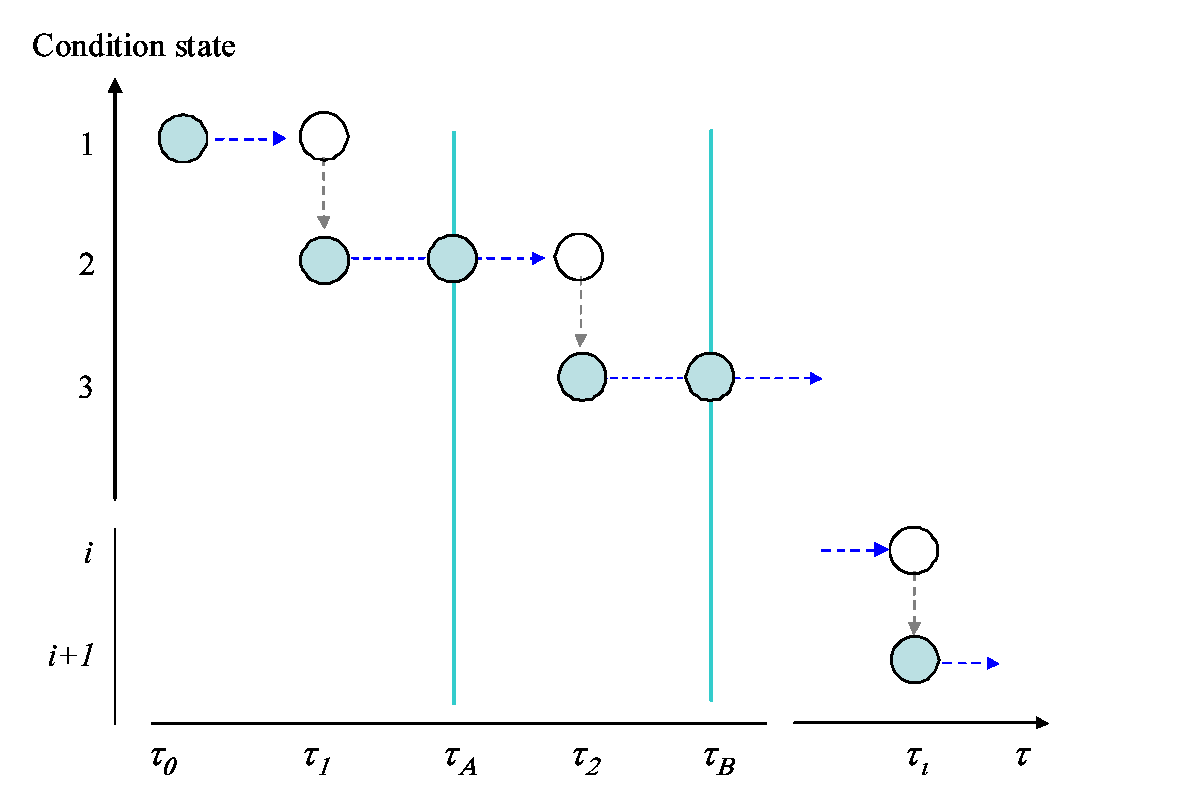
\includegraphics[scale=0.5]{fig23} 
\end{center}
\footnotesize Note) In this example, the deterioration process of a infrastructure component if expressed in terms of calendar time $\tau_1, \tau_2,...,\tau_i$, and condition state of the section is increased in unitary units.
\caption{Transition Time of Condition State.}
\label{fig23} 
\end{figure}
%%
%
Information regarding the deterioration process of an infrastructure can be acquired through periodical visual inspections. However, information on the condition state based on continuous visual inspection is difficult to obtain. In this case, the initial inspections is carried out at times $\tau_A$ on the time-axis. It is supposed that at time $\tau_A$ the condition state observed by inspection is $i~(i=1,\cdots,J-1)$. The deterioration progress in future times is uncertain. Among the infinite set of possible scenarios describing the deterioration process only one path is finally realized. 

Figure \ref{fig24} shows four possible sample paths. Path 1 shows no transition in the condition state $1$ from initial time $\tau_0$ to first inspection time $\tau_A$. In paths 2 and 3, condition state has advanced to one upper state condition at the calendar times $\tau_1^2$ and $\tau_1^3$ respectively. The condition state of these two paths observed at time $\tau_A$ become $2$. In a periodical inspection scheme, the point times $\tau_1^2$ and $\tau_1^3$ in which the condition state has changed from $1$ to $2$ are not determined. In addition, path 4 shows transitions in the condition state at times $\tau_i^4$ and $\tau_{i+1}^4$ during the inspection interval. The condition state observed at time $\tau_A$ becomes $3$. That is, in spite of the transitions in the condition state are observable at the time of periodical inspection, it is not possible to obtain information about the times in which those transitions occur.

Figure \ref{fig25} further describes the deterioration process inferring the inspection approach and how the condition state is assumed. In this figure, it is assumed that the condition state at the calendar time $\tau_{i-1}$ has changed from $i-1$ to $i$. The calendar time $\tau_{i-1}$ is assumed to be equivalent to $y_i=0$. The time represented by the sample time-axis is referred from now on as a ``time point'', and differs from ``time'' on the calendar time axis. The times $\tau_A$ and $\tau_B$ correspond to the time points $y_A$ and $y_B$ on the sample axis. It can be seen that $y_A=\tau_A-\tau_{i-1}$, $y_B=\tau_B-\tau_{i-1}$. 

Information on the condition state $i$ at the beginning of the calendar time $\tau_{i-1}$ cannot be obtained in a periodical inspection scheme. Therefore, time points $y_A$ and $y_B$ on the sample time-axis cannot be correctly obtained either. For convenience of description, it is assumed that the information at the time a point is known in order to develop the model, despite this assumption is not necessarily essential. The following paragraph discusses that even without information at time points $y_A$ and $y_B$ an exponential hazard model can be estimated.
\begin{figure}[t]
\begin{center}
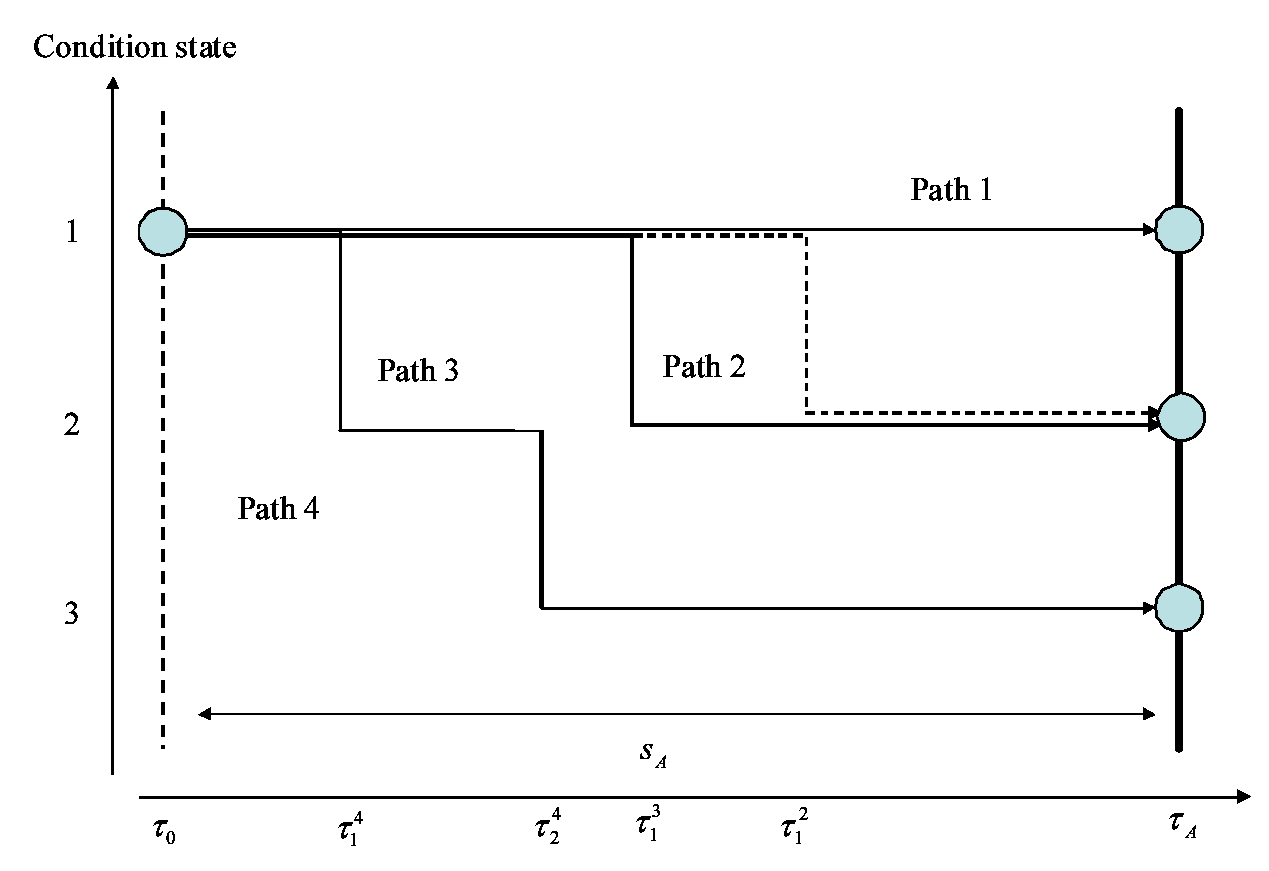
\includegraphics[scale=0.5]{fig24} 
\end{center}
\footnotesize Note) In this example, the deterioration process of an infrastructure component is expressed in terms of four different sample paths. In paths 2 and 3 the condition state has advanced to one upper state condition at the calendar times $\tau_1^2$ and $\tau_1^3$ respectively. In path 4, the condition state has increased one state at each time $\tau_1^4$ and $\tau_{2}^4$. However, in the case of a periodical inspection carried out at times $\tau_A$ the condition state at any point in time between inspections cannot be observed.
\caption{Transition Pattern of Condition State.}
\label{fig24} 
\end{figure}

In the case the condition state of a infrastructure component at time $\tau_{i}$ (time point $y_C$) is assumed to change from $i$ to $i+1$, the period length in which the condition state has remained at $i$ (referred as the life expectancy of a condition state $i$) is represented by $\zeta_i=\tau_{i}-\tau_{i-1}=y_C$. The life expectancy of a condition state $i$ is assumed to be a stochastic variable $\zeta_i$ with probability density function $f_i(\zeta_i)$ and distribution function $F_i(\zeta_i)$. Random variable $\zeta_i$ is defined in the domain $[0,\infty]$. The distribution function is defined as
\begin{eqnarray}
&& F_i(y_i)=\int_0^{y_i}f_i(\zeta_i)d\zeta_i. \label{func21}
\end{eqnarray}
\begin{figure}[t]
\begin{center}
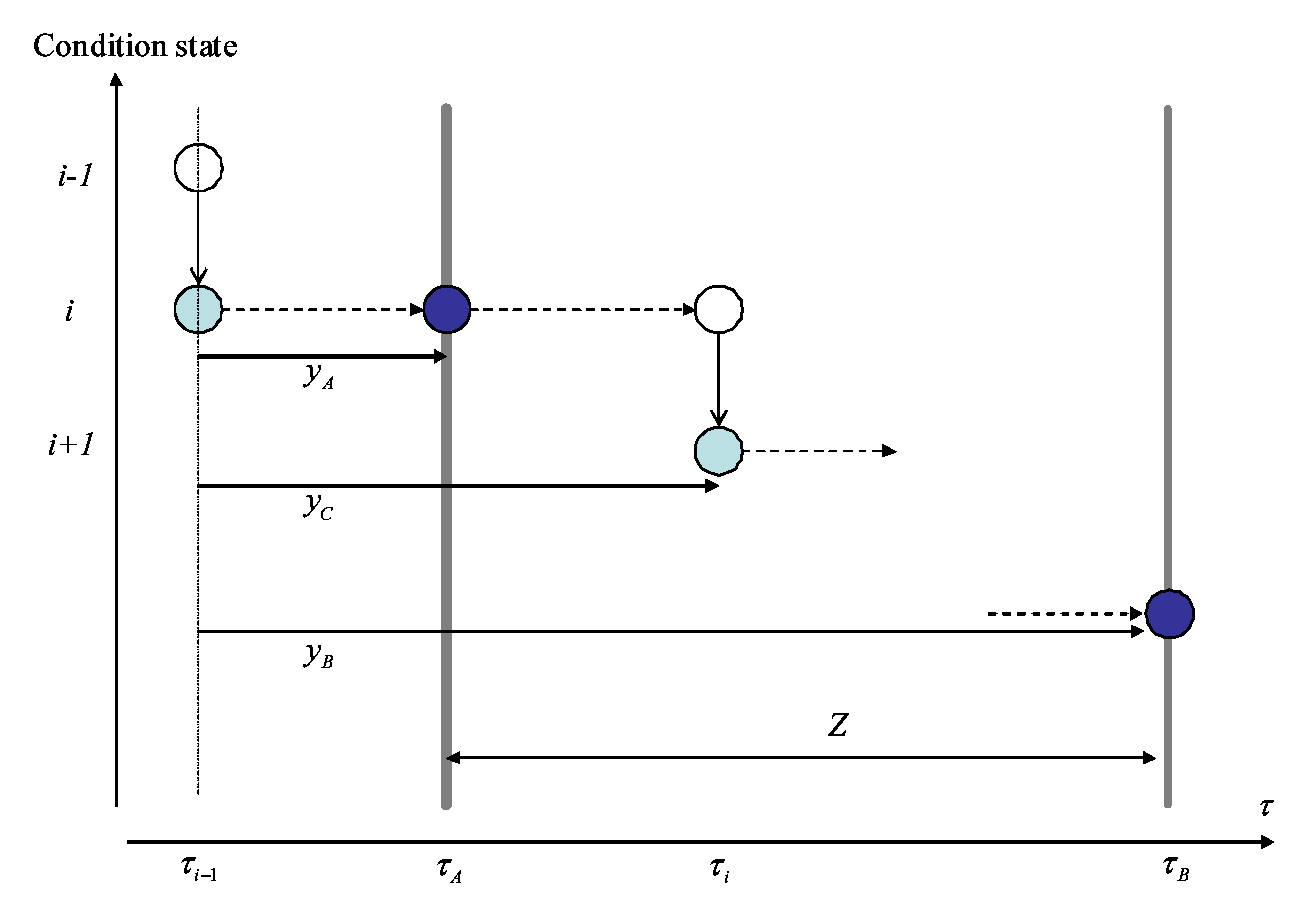
\includegraphics[scale=0.5]{fig25} 
\end{center}
\footnotesize Note) In the case the condition state changes from $i-1$ to $i$ at the calendar time $\tau_{i-1}$ the inspections carried out at times $\tau_A$ and $\tau_B$ will also correspond to the points in time $y_A$ and $y_B$ when using $\tau_{i-1}$ as the time origin. The figure shows a sample deterioration path in which the condition state has advanced in one unit to $y_c$ in the interval time $\tau_{i-1}-y_C$. However, observations at time $\tau_{i-1}$ are not possible in a periodical inspection scheme, so there is no way to obtain observation at $y_A$, $y_B$ and $y_C$. Nevertheless, it is possible to use the information contained in $z=y_C-y_A \in [0,Z]$.
\caption{Model of Deterioration Process.}
\label{fig25} 
\end{figure}

The distribution function $F_i(y_i)$ represents the cumulative probability of the transition in the condition state from $i$ to $i+1$. Condition state $i$ is assumed to be observed at initial time $y_i=0$(time $\tau_A$). The time interval measured along the sample time-axis until the time point $y_i$ is $\tau_{i-1}+y_i$. Therefore, using the cumulative probability $F_i(y_i)$, the probability $\tilde{F}_i(y_i)$ of a transition in the condition state $i$ during the time points interval $y_i=0$ to $y_i\in [0,\infty]$ is defined by $\tilde{F}_i(y_i)$:
\begin{eqnarray}
&& \mbox{Prob}\{\zeta_i \geq y_i\}= \tilde{F}_i(y_i) = 1 -  F_i(y_i). \label{funcbF}
\end{eqnarray}
The conditional probability that the condition state of a component at time $y_i$ advances from $i$ to $i+1$ during the time interval $[y_i,y_i+\Delta y_i]$ is defined as
\begin{eqnarray}
&& \lambda_i(y_i) \Delta y_i = \frac{f_i(y_i)\Delta y_i}{\tilde{F}_i(y_i)}  \label{riskbF},
\end{eqnarray}
where the probability density $\lambda_i(y_i)$ is referred as the hazard function.
%%%%%%%%%%%%%%
\subsection{Markov Transition Probability}
\label{232}
The transition process among the condition states of an infrastructure component is uncertain. Therefore, future condition states cannot be forecasted deterministically. In this situation, Markov transition probability is employed to represent the uncertain transition pattern of the condition states during two time points. Markov transition probabilities can be defined for arbitrary time intervals. 

For simplification, Markov transition probabilities can be defined and used to forecast the deterioration of a infrastructure component based on the information from periodical inspection scheme shown in Figure \ref{fig25}. The observed condition state of the component at time $\tau_A$ is expressed by using the state variable $h(\tau_A) $. If the condition state observed at time $\tau_A$ is $i$, then the state variable $h(\tau_A)=i$. A Markov transition probability, given a condition state $h(\tau_A) =i$ observed at time $\tau_A$, defines the probability that the condition state at a future time ($\tau_B$ for example) will change to $h(\tau_B) =j$:
\begin{eqnarray}
&& \mbox{Prob}[h(\tau_B)=j|h(\tau_A)=i]=\pi_{ij}.\label{pro}
\end{eqnarray}
The Markov transition probability matrix can be defined and rearranged by using the transition probabilities between each pair of condition states $(i,j)$ as
\begin{eqnarray}
&& {\bf \Pi}=\left(
\begin{array}{ccc}
\pi_{11} & \cdots & \pi_{1J} \\
\vdots & \ddots & \vdots \\
0 & \cdots & \pi_{JJ}
\end{array}
\right). 
\end{eqnarray}
The Markov transition probability (\ref{pro}) shows the transition probability between the condition states at two given times $\tau_A$ and $\tau_B$, therefore, it is straightforward that the values of a transition probability will differ for different time intervals. Since deterioration continues as long as no repair is carried out $\pi_{ij}=0~(i>j)$. From the definition of transition probability $\sum^{J}_{j=1}\pi_{ij}=1$. Following conditions must be satisfied:
\begin{eqnarray}
\left.
\begin{array}{l}
\pi_{ij}\geq 0 \\
\pi_{ij}=0 \,\,~(\,\mbox{when} \,\,\, i>j) \\
\sum_{j=1}^J \pi_{ij}=1 \\
\end{array}
\right\}.\label{suii}
\end{eqnarray}
The worse level of deterioration is expressed by the condition state $J$, which remains as an absorbing state in the Markov chain as long as no repair is carried out. In this case $\pi_{JJ}=1$.

Markov transition probabilities are defined independently from the deterioration history. As shown in Figure \ref{fig25}, the condition state at the inspection time $\tau_A$ is $i$, however, the time, at which, condition state changed from $i-1$ to $i$ is unobservable. In a Markov chain model, it is assumed that the transition probability between the inspection times $\tau_A$ and $\tau_B$ is only dependent on the condition state at time $\tau_A$. 

The Markov chain model is operative and widely applied in management of infrastructure system. Particularly, at management of network level, Markov chain model is used to define the average transition probability of the entire system, or a group of infrastructure components given two periodical inspection data.
%%%%%%%%%%%%%%%%%%%%%%%%
\subsection{Exponential Hazard Model}
\label{233}
%%%%%%%%%%%%%%%%%%%%%%%%%%%%%%%%%%
In this section, it is assumed that the deterioration of a infrastructure component satisfies Markov property, and the hazard function is independent of the time $y_i$ on the time-axis. That is, for a fixed value of $\theta_i>0$, we have
\begin{eqnarray}
&& \lambda_i(y_i)=\theta_i \hspace{2mm}. \label{hazard}
\end{eqnarray}
By using the hazard function (\ref{hazard}), it is possible to represent a deterioration process of a infrastructure component that satisfies the Markov property (Independence from the past history). In addition, it is assumed that $\theta_i\neq \theta_j~(i \neq j)$. By differentiating both sides of equation (\ref{funcbF}) with respect to $y_i$,
\begin{eqnarray}
&& \frac{d\tilde{F}_i(y_i)}{dy_i}=-f_i(y_i).\label{op}
\end{eqnarray}
Equation (\ref{riskbF}) then becomes
\begin{eqnarray}
&& \lambda_i(y_i) = \frac{f_i(y_i)}{\tilde{F}_i(y_i)} =-\frac{\frac{d\tilde{F}_i(y_i)}{dy_i}}{\tilde{F}(y_i)} 
= \frac{d}{dy_i}\left( - \log \tilde{F}_i(y_i) \right).\label{opi}
\end{eqnarray}
Considering that $\tilde{F}_i(0)=1-F_i(0)=1$, and by integrating equation (\ref{opi}), we come up with
\begin{eqnarray}
&& \hspace{-9mm} \int_{0}^{y_i} \lambda_i(u)du = \big[-\log \tilde{F}_i(u)\big]_{0}^{y_i} = -\log \tilde{F}_i(y_i).
\end{eqnarray}
Using the hazard function $\lambda_i(y_i)=\theta_i$, the probability $\tilde{F}_i(y_i)$ that the life expectancy of the condition state $i$ becoming longer than $y_i$ is expressed by
\begin{eqnarray}
&& \tilde{F}_i(y_i) = \exp \left[ - \int_{0}^{y_i}\lambda_i(u)du \right] 
 = \exp (-\theta_i y_i). \label{prop-bFla}
\end{eqnarray}
Equation (\ref{prop-bFla}) is exponential form of hazard model. According to equation (\ref{op}), the probability density function $f_i(\zeta_i)$ of the life expectancy of the condition state $i$ is
\begin{eqnarray}
&& f_i(\zeta_i)=\theta_i \exp(-\theta_i \zeta_i).\label{kikan}
\end{eqnarray}
By then, considering that the condition state has changed to $i$ at the time  $\tau_{i-1}$, and remains constant until the inspection time $\tau_A$. Obvious to say, the condition state observed at inspection time $\tau_A$ is $i$. In term of duration, condition state $i$ has actually stayed in the period $y_A$. The probability, to which the condition state $i$ keeps remaining in a subsequent time $z_i~(\geq 0)$ measured after the duration $y_A$, is then defined:
\begin{eqnarray}
&& \tilde{F}_i(y_A+z_i|\zeta_i \geq y_A) 
 = \mbox{Prob} \{\zeta_i \geq y_A+z_i | \zeta_i \geq y_A\}. \label{eq213}
\end{eqnarray}
Dividing both sides of equation (\ref{eq213}) by the probability $\tilde{F}_i(y_i)$ described in equation (\ref{funcbF}) results in
\begin{eqnarray}
&& \frac{\mbox{Prob} \{\zeta_i \geq y_A+z_i\}}{ \mbox{Prob}\{\zeta_i \geq y_A\}} = \frac{\tilde{F}_i(y_A+z_i)}{\tilde{F}_i(y_A)}. \label{eq214}
\end{eqnarray}
With reference to equation (\ref{prop-bFla}), the right side of equation (\ref{eq214}) becomes:
\begin{eqnarray}
&& \frac{\tilde{F}_i(y_A+z_i)}{\tilde{F}_i(y_A)}= \frac{\exp \{-\theta_i (y_A+z_i)\}}{\exp( - \theta_i y_A)} 
 =\exp (-\theta_i z_i). \label{eq215}
\end{eqnarray}
Based on this conditional rule, we can define the probability, to which, the condition state $i$ observed at time $\tau_A$ continues to be observed at subsequent inspection time $y_B=y_A+Z$ is analogous to equation (\ref{eq215}):
\begin{eqnarray}
&& \hspace{-3mm} \mbox{Prob}[h(y_B)=i|h(y_A)=i]=\exp(-\theta_i Z), \label{pro1},
\end{eqnarray}
where $Z$ expresses the interval between two inspection times. The probability $\mbox{Prob}[h(y_B)=i|h(y_A)=i]$ is nothing but the Markov transition probability $\pi_{ii} $. Obviously, if the exponential hazard function is employed, the transition probability $\pi_{ii} $ is dependent only on the hazard rate $\theta_i$ and the inspection interval $Z$.
%Even more, without using deterministic information on the time points $y_A$ and $y_B$, it is still possible to estimate transition probabilities.
%%%%%%%%%%%%%%%%%%%%%%%%%%55
\subsection{Weibull Hazard Model}
\label{234}
In reality, the data concerning deterioration of infrastructure facilities are not only condition state but also their embedded characteristics. This information can be observed from inspections. However, in actual practices, the inspection intervals of different infrastructure, components do not possess the same duration. In this respect, Markov chain model using only two recent inspection data might not reflect overall performance. Weibull hazard function can capture the historical performance is thus beneficial in this circumstance. 

The assumption of deterioration can be referred to Figure \ref{fig26}. In this figure, condition state starts to change from $i-1$ to $i$ at time $\tau_{i-1}$. $y_i$ is elapsed time or duration of stay in condition state $i$. The duration $y_A$ is estimated by $y_A = \tau_A - \tau_{i-1}$ and understood as the elapsed time between calendar time $\tau_{i-1}$ and $\tau_A$.

\begin{figure}[t]
\begin{center}
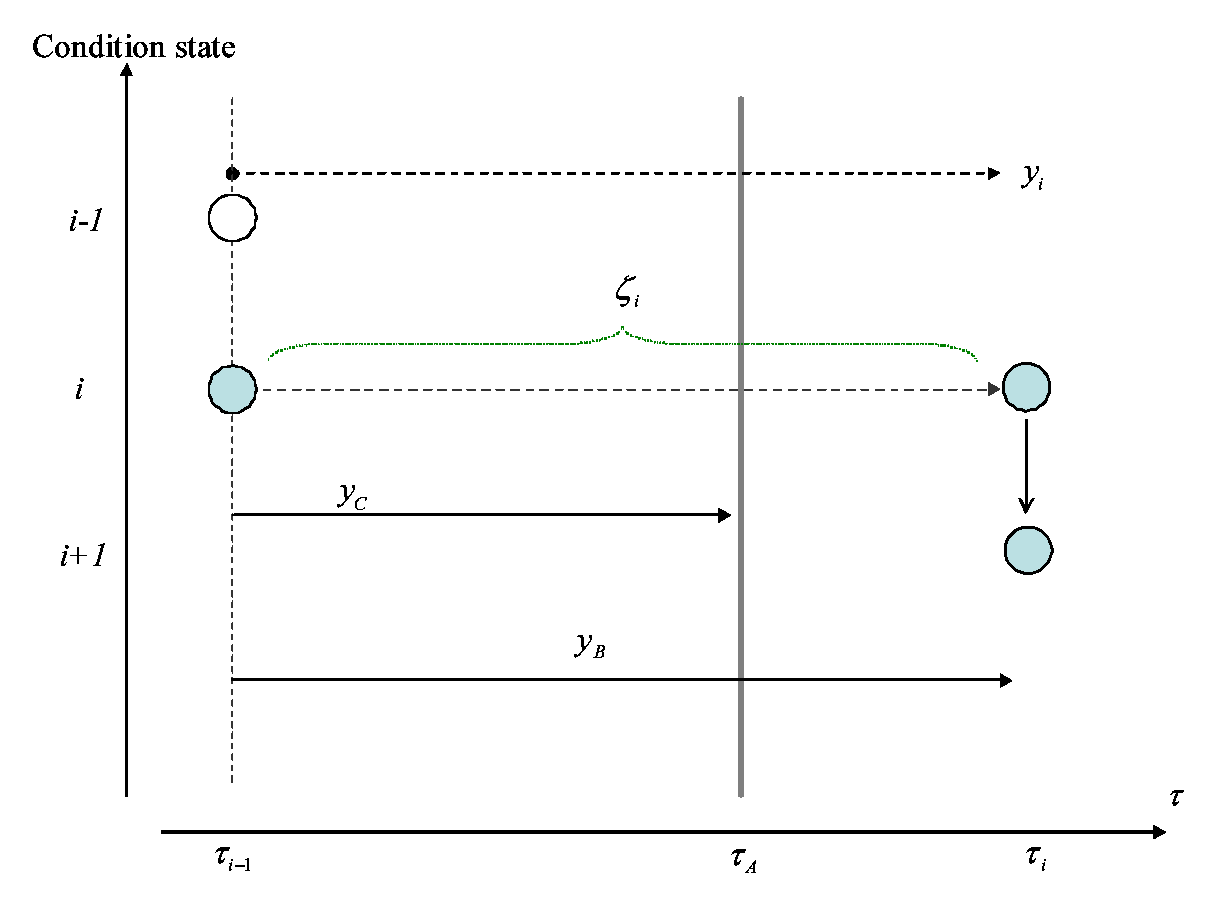
\includegraphics[scale=0.5]{fig26} 
\end{center}
\footnotesize Note) Condition state changes from $i-1$ to $i$ at calendar time $\tau_{i-1}$, which refers as starting point of deterioration process. The inspection is carried out at time $\tau_A$ and at which we have corresponding time length $y_A$ counted from $\tau_{i-1}$. The condition state continues to occupy length $y_B$ in its deterioration path. However, at time $\tau_{i-1}$, there is no observation. In the sequel, the exact time length $y_A$ and $y_B$ on the time axis can not be determined.
\caption{Condition State and Inspection Interval.}
\label{fig26} 
\end{figure}
%%%
From equations (\ref{func21}-\ref{riskbF}), applying similar mathematical approach like in equations (\ref{op}-\ref{pro1}), in the form of Weibull distribution, hazard function $\lambda_i$, survival probability $\tilde{F} _ i(y_i)$ and probability density function $f_i(\zeta_i)$ can be expressed: 
\begin{eqnarray}
&& \lambda_i(y_i)= \theta_i \alpha_{i} y_i^{\alpha_{i}-1}, \label{hazardw}\\
&& \tilde{F}_i(y_i) = \exp (-\theta_i y_i^{\alpha_{i}}), \label{prop-bFlaw}\\
&& f_i(\zeta_i)=\theta_i \alpha_{i} \zeta^{\alpha_{i}-1}_i\exp(-\theta_i \zeta^{\alpha_{i}}_i).\label{kikanw}
\end{eqnarray}
%%%%%%%%%%%%%
\section{Deterioration Hazard Model Estimation Method}
\label{24}
\subsection{Exponential hazard model}
\label{241}
\subsubsection{Defining Markov transition probabilities}
\label{2411}
This section continues the formation of transition probability earlier explained in section \ref{232} and section \ref{233} for general case.

Let us discuss the formulation of model in the case condition state $i$ advancing in only one-step, to condition state $i+1$ in the inspection interval from $\tau_A$ to $\tau_B$. At first, it is assumed that condition state $i$ remains during duration $y_A$ and in subsequent increment of time $s_i=y_A+z_i, (z_i\in [0,Z])$. Secondly, condition state $i$ changes into $i+1$ at $y_A+z_i$. Thirdly, condition state $i+1$ keep unchanging during the interval $[y_A+z_i$, $y_B]$.

Although the exact time, at which the condition state transits from $i$ to $i+1$ can not be traced by periodical inspection, it can be temporarily assumed that the transition occurs at the time point $(y_A+\bar{z}_i) \in [y_A,y_B]$. Given the condition state $i$ staying during $y_A$ and remains until the time $y_A+\bar{z}_i$, the conditional probability density, to which condition state $i+1$ being observed at $y_A+\bar{z}_i$ can be defined:
\begin{eqnarray}
&& \hspace{-8mm} g_i(\bar{z}_i|\zeta_i \geq y_A)=\frac{f_i(\bar{z}_i+y_A)}{\tilde{F}_i(y_A)} 
 =\frac{\theta_i \exp\{-\theta_i (\bar{z}_i+y_A)\}}{\exp(-\theta_i y_A)}
=\theta_i \exp(-\theta_i \bar{z}_i).
\end{eqnarray}
Satisfying the above condition, the conditional probability density that the condition state $i+1$ being observed at the inspection time $y_B$ becomes:
\begin{eqnarray}
&& \hspace{-3mm} q_{i+1}(\bar{z}_i|\zeta_i\geq y_A) 
 = g_i(\bar{z}_i|\zeta_i \geq y_A) \cdot \tilde{F}_{i+1}(y_B-\bar{z}_i-y_A) \nonumber\\
&& = \theta_i \exp(-\theta_i \bar{z}_i) \exp\{-\theta_{i+1}(Z-\bar{z}_i)\} \nonumber\\
&& = \theta_i \exp(-\theta_{i+1}Z)\exp\{-(\theta_i-\theta_{i+1})\bar{z}_i\}.
\end{eqnarray}
It is noticed that $\bar{s}_i=y_A+\bar{z}_i$ is assumed as fixed value. However, the elapsed time $\zeta_i$ of a condition state $i$ is truly a stochastic variable, thus,  $\bar{z}_i$ may change in range $[0, Z] $. The Markov transition probability that the condition state change from $i$ to $i+1$ during the time points $y_A$ and $y_B$ is then defined by the law of integration:
\begin{eqnarray}
&& \hspace{-5mm} \pi_{ii+1}=\mbox{Prob}[h(y_B)=i+1|h(y_A)=i] 
 =\int_{0}^{Z} q_{i+1}(z_i|\zeta_i\geq y_A)dz_i \nonumber \\
&& \hspace{-3mm} =\int_0^{Z} \theta_i \exp(-\theta_{i+1}Z)\exp\{-(\theta_i-\theta_{i+1})z_i\}dz_i \nonumber \\
&& \hspace{-3mm} = \frac{\theta_i}{\theta_{i}-\theta_{i+1}}\{-\exp(-\theta_{i}Z)+\exp(-\theta_{i+1}Z)\},\label{iik}
\end{eqnarray}
where $\pi_{ii+1}>0$ is indifferent to the relative size between $\theta_i$ and $\theta_j$. The assumption $\theta_i\neq \theta_{i+1}$ implies $1>\pi_{ii+1}$. As these characteristics are trivial in the derivation process of equation (\ref{iik}), the verification is omitted. 

Moving to general case, when in the next inspection, condition state $j(j\geq i +2)$ is observed. The distribution function and the probability density function concerning the duration condition state $j$ actually stays in can be assumed as $F_j(y_j) $ and $f_j(y_j)$. The hazard function applying on the condition state $j$ is denoted by $\lambda_j(y_j) =\theta_j$. 

The process, where by happening the transition of condition state from $i$ to $i+1$ during interval $[y_A,y_B]$ can be perceived as follows. At first, the condition state $i$ remains during the elapsed time $y_A$ and in a subsequent time $\bar{s}_i=y_A+\bar{z}_i \in [y_A,y_B]$. Secondly, exactly at time $\bar{s}_i=y_A+\bar{z}_i$, condition state $i$ changes into $i+1$. Thirdly, condition state $i+1$ remains in the duration $[\bar{s}_i=y_A+\bar{z}_i, \bar{s}_{i+1}=\bar{s}_{i}+\bar{z}_{i+1}~(\leq y_B)]$ before turning to condition state $i+2$ at $\bar{s}_{i+1}=\bar{s}_{i}+\bar{z}_{i+1}$. Fourthly, after repeating the same transition process, condition state happens to change into $j$ at time $\bar{s}_{j-1}~(\leq y_B)$, and keep unchanging until inspection time $y_B$. If the entire process of transition is considered, a simultaneously conditional probability density function can be defined as follow:
\begin{eqnarray}
&& q_{j}(\bar{z}_i,\bar{z}_{i+1},\cdots,\bar{z}_{j-1}|\zeta_i\geq y_A) \nonumber \\
&& = g_i(\bar{z}_i|\zeta_i \geq y_A) \prod_{m=i+1}^{j-1} f_{m}(\bar{z}_m) \tilde{F}_{j}\left(Z-\sum_{m=i}^{j-1} \bar{z}_m\right)
\nonumber\\
&& = \prod_{m=i}^{j-1}\theta_m\cdot \exp\left\{- \sum_{m=i}^{j-1} \theta_m \bar{z}_m -\theta_{j}(Z-\sum_{m=i}^{j-1} \bar{z}_m)\right\}\nonumber \\
&& = \prod_{m=i}^{j-1}\theta_m \cdot \exp\left\{-\theta_j Z - \sum_{m=i}^{j-1} (\theta_m-\theta_{j})\bar{z}_m\right\},
\end{eqnarray}
where $\bar{z}_i,\cdots,\bar{z}_{j-1}$ are regarded as fixed values. However, the elapsed time $\zeta_i$ of condition states $i~(i=1,\cdots,J-1)$ is a stochastic variable, the values of $z_i\geq 0,\cdots,z_{j-1}\geq 0$ are variable, which subject to satisfy the following condition:
\begin{eqnarray}
&& 0\leq z_i+z_{i+1}+\cdots+z_{j-1}\leq Z.
\end{eqnarray}
As the sequent, for continuous observed time, the Markov transition probabilities $\pi_{ij}$ is conditional probability and being described in following equation:
\begin{eqnarray}
&& \hspace{-10mm} \pi_{ij}=\mbox{Prob}[h(y_B)=j|h(y_A)=i] 
 =\int_{0}^{Z}\int_0^{Z-z_i} \cdots \int_{0}^{Z-\sum_{m=i}^{j-2}z_{m}}\nonumber \\
&& \hspace{-5mm} q_{j}(z_i,\cdots,z_{j-1}|\zeta_i\geq y_A)dz_i\cdots dz_{j-1} \nonumber \\
&& \hspace{-10mm} =\sum_{k=i}^{j}\prod_{m=i}^{k-1}\frac{\theta_m}{\theta_{m}-\theta_{k}}\prod_{m=k}^{j-1}\frac{\theta_m}{\theta_{m+1}-\theta_{k}}\exp(- \theta_{k} Z). \label{dousyutu}
\end{eqnarray}
Details of description for getting into equation (\ref{dousyutu}) is given in the paper of \citet{kobayashitsuda}. For convenient reading, general forms of Markov transition probabilities are given in the following equations:
\begin{manyeqns}
&& \pi_{ii}=\exp(-\theta_i Z), \label{p1} \\
&& \pi_{ii+1}= \frac{\theta_i}{\theta_{i}-\theta_{i+1}}\{-\exp(-\theta_{i}Z)+\exp(-\theta_{i+1}Z)\}, \\
&& \pi_{ij}= \sum_{k=i}^{j}\prod_{m=i}^{k-1}\frac{\theta_m}{\theta_{m}-\theta_{k}}\prod_{m=k}^{j-1}\frac{\theta_m}{\theta_{m+1}-\theta_{k}}\exp(- \theta_{k} Z) \label{hazardpiij}, \\
&& \pi_{iJ}=1-\sum_{j=i}^{J-1}\pi_{ij}, \label{pj}\\
&& \hspace{5mm} (i=1,\cdots,J-1) \hspace{5mm} (j=i,\cdots,J). \nonumber
\end{manyeqns}
%%%%
\subsubsection{Time adjustment of Markov transition probability}
\label{2412}
%%%%
Markov transition probabilities depend on the inspection interval $Z$ as can be revealed from equations (\ref{p1}) - (\ref{pj}). In cardinal matrix form, we can further expressed the time interval depend of Markov transition probability:
\begin{eqnarray}
&& \mbox{\boldmath$\Pi$}(Z)=\left(
\begin{array}{ccc}
\pi_{11}(Z) & \cdots & \pi_{1J}(Z) \\
\vdots & \ddots & \vdots \\
0 & \cdots  & \pi_{JJ}(Z)
\end{array}
\right).
\end{eqnarray}
Inspections are scheduled in a regular based time with integer number $n$. If two inspection interval $Z$ and $nZ$ are considered, the two Markov transition probability matrix $\mbox{\boldmath$\Pi$} (Z) $ and $\mbox{\boldmath$\Pi$} (nZ) $ can also be used to express the dependency on inspection interval. Based on the law of matrix multiplication, the relation between $\mbox{\boldmath$\Pi$} (Z) $ and $\mbox{\boldmath$\Pi$} (nZ) $ is clearly defined:
\begin{eqnarray}
&& \mbox{\boldmath$\Pi$}(nZ)=\left\{\mbox{\boldmath$\Pi$}(Z)\right\}^n .\label{seigou}
\end{eqnarray}
Equation (\ref{seigou}) expresses the time adjustment condition of the Markov transition probability matrix. If $n$ becomes very big number, a stationary state of transition probabilities will be obtained. It is concluded here that with respect to different time interval $Z$, we can adjust the properties of Markov transition probability to reflect the actual inspection schedule in practices.
%%%%%%%%%%
\subsubsection{Estimation of Markov Transition Probability}
\label{2413}
\textit{(a) Contents of periodical inspection data}

Suppose periodical inspection data on the same kind of $K$ infrastructure components is available. An inspection sample $k(k= 1, \cdots, K) $ describes two continuous periodical inspections carried out at times $\tau_A^k$ and $\tau_B^k$ and the respective condition states ratings $h(\tau_A^k)$ and $h(\tau_B^k)$ measured at those times. Differences in the inspection intervals of the samples are inconvenient. Based on the above inspection data, the inspection interval of a sample $k$ is defined as $Z^k=\tau_B^k-\tau_A^k$. In addition a dummy variable $\delta_{ij}^k~(i,j=1,\cdots,J; k=1,\cdots,K)$ based on the deterioration progress patterns between two inspections times is defined as
\begin{eqnarray}
&& \hspace{-8mm} \delta_{ij}^k=\left\{
\begin{array}{ll}
1 & \mbox{when} \;\,h(\tau_A^k)=i \;\,\mbox{and}\;\, h(\tau_B^k)=j\\
0 & \mbox{otherwise}
\end{array}.
\right.
\end{eqnarray}
Furthermore, the structural characteristics and usage conditions that affect the deterioration of an infrastructure component are represented by the vector $\mbox{\boldmath$x$}^k=(x_1^k,\cdots,x_M^k)$. $x_m^k~(m=1,\cdots,M)$ represents the value of a characteristic variable $m$ observed in the sample data $k$. The information contained in the inspection sample data $k$ can be rearranged as $\Xi^k=(\delta_ {ij} ^k, Z^k, \mbox{\boldmath$x$}^k) $. On the other hand, the exponential hazard function of the deterioration process for a sample data $k(k= 1, \cdots, K) $ is 
\begin{eqnarray}
&& \lambda_i^k(y_i^k)=\theta_i^k ~(i=1,\cdots,J-1). \nonumber
\end{eqnarray}
It is noted here that the hazard rate for condition state $J$ is not defined because $J$ is absorbing condition state ($\pi_{JJ} =1$). The hazard rate $\theta_i^k~(i=1,\cdots,J-1;k=1,\cdots,K)$ characterizing the deterioration process is considered to change in relation to the vector $\mbox{\boldmath$x$}^k$ as follow: 
\begin{eqnarray}
&& \theta_i^k=\mbox{\boldmath$x$}^k\mbox{\boldmath$\beta$}_i^\prime ,\label{hazard1}
\end{eqnarray}
where $\mbox{\boldmath$\beta$}_i=(\beta_{i,1},\cdots,\beta_{i,M})$ is a row vector of unknown parameters $\beta_{i,m}~(m=1,\cdots,M)$ and the symbol $\prime$ indicates the vector is transposed. In order to obtain Markov transition probabilities, at first, the exponential hazard function $\lambda_i^k(y_i^k)=\theta_i^k$ is estimated based on the observed sampling information $\Xi^k~(k=1,\cdots,K)$. Secondly, Markov transition probabilities can be estimated based on the relation with hazard function. 

This methodology permits estimation for Markov transition probabilities of every individual infrastructure component. However, as a rule of thumb, it is better to estimate the average transition probability for the entire group of infrastructure instead of estimating for individual component. 

\textit{(b) Infrastructure management indicators}

Using exponential hazard model, we can define one of the important management indicator for infrastructure. The indicator is the remaining duration ($RMD_i$) of condition state $i$, which reflects how long condition state $i$ can survive given condition that it has been observed in previous inspection time. $RMD_i$ is actually analogous to survival function $\tilde{F}_i(y_i^k)$ in infinite domain \cite{lancaster90}:
\begin{eqnarray}
&& RMD_i^k= \int^{\infty}_{0}\tilde{F}_i(y_i^k)dy_i^k \hspace{1mm}.\label{17}
\end{eqnarray}
Based on equation (\ref{prop-bFla}), the remaining duration $RMD^k_i$ of component $k$ can be further defined in the exponential form:
\begin{eqnarray}
&& RMD_i^k= \int^{\infty}_{0}\exp (-\theta_i^k y_i^k) dy_i^k = \frac{1}{\theta_i^k} \hspace{1mm}.\label{rating}
\end{eqnarray}
Assuming the condition state after opening the infrastructure is $i$. The expected value $ET_j~(j=2,\cdots,J)$ referred as average life expectancy of condition state $j$, is thus a summation of all transition duration from every condition state $i$:
\begin{eqnarray}
&& ET_j=\sum_{i=1}^j \frac{1}{\lambda_i}\hspace{1mm}. \label{hy}
\end{eqnarray}
Rating $j~(j=1\cdots,J)$ and average relation of elapsed time $ET_j(\mbox{\boldmath$x$})$  are used to draw the expectation deterioration curve.
%%%%%%%%%%%%

\textit{(c) Estimation of the hazard model}

Information $\Xi^k=(\bar{\delta}_{ij}^k,\bar{Z}^k,\bar{\mbox{\boldmath$x$}}^k)$ can be acquired in relation to the inspection sample $k$, where the symbol $\bar{}$ indicates an actual measurement. The Markov transition probabilities can be expressed in terms of the hazard functions as described in equations (\ref{p1})-(\ref{pj}). The relationship between hazard rate $\theta_i^k~(i=1,\cdots,J-1;k=1,\cdots,K)$ and the characteristic variables $\bar{\mbox{\boldmath$x$}}^k$ is shown in equation (\ref{hazard1}). Moreover, the transition probability also depends on inspection interval $\bar{Z}^k$.

For clarity of presentation, the transition probability $\pi_{ij}$ is expressed as a function of the measured data $(\bar{Z}^k,\bar{\mbox{\boldmath$x$}}^k)$ obtained from visual inspection and the unknown parameters $\mbox{\boldmath$\beta$}_i$ as $\pi_{ij}(\bar{Z}^k,\bar{\mbox{\boldmath$x$}}^k:\mbox{\boldmath$\beta$}_i)$. If the deterioration progress of the infrastructure components in a sample $K$ are assumed to be mutually independent, the log-likelihood function expressing the simultaneous probability density of the deterioration transition pattern for all inspection samples is \cite{tobin,amemi}
\begin{eqnarray}
&& \hspace{-3mm} \ln[{\cal L}(\mbox{\boldmath$\beta$})] = \ln \left[\prod_{i=1}^{J-1} \prod_{j=i}^J\prod_{k=1}^{K} \left\{\pi_{ij}(\bar{Z}^k,\bar{\mbox{\boldmath$x$}}^k:\mbox{\boldmath$\beta$})\right\}^{\bar{\delta}_{ij}^k}\right]
\nonumber \\
&& \hspace{5mm} =\sum_{i=1}^{J-1} \sum_{j=i}^J\sum_{k=1}^K \bar{\delta}_{ij}^k \ln\left[
\pi_{ij}(\bar{Z}^k,\bar{\mbox{\boldmath$x$}}^k:\mbox{\boldmath$\beta$})\right] \hspace{1mm},
 \label{logbF}
\end{eqnarray}
where $\bar{\delta}_{ij}^k$, $\bar{Z}^k$ and  $\bar{\mbox{\boldmath$x$}}^k$ are all determined through inspections, and $\mbox{\boldmath$\beta$}_i~(i=1,\cdots,J-1)$ are parameters to be estimated. Estimations of the parameters $\mbox{\boldmath$\beta$}$ can be obtained by solving the optimality condition:
\begin{eqnarray}
&& \frac{ \partial \ln[{\cal L}(\hat{\mbox{\boldmath$\beta$}})] }{\partial \beta_{i,m}}=0, \label{saiteki}
\hspace{3mm} \quad ~(i=1,\cdots,J-1;m=1,\cdots,M) \hspace{1mm}
\end{eqnarray}
that result from maximizing the log-likelihood function (\ref{logbF}). The optimal values $\hat{\mbox{\boldmath$\beta$}}=(\hat{\beta}_{1,1},\cdots,\hat{\beta}_{J,M})$ are then estimated by applying a numerical iterative procedure such as the Newton Method for the $(J-1)M$ order nonlinear simultaneous equations \cite{isoda}. Furthermore, estimator for the asymptotic covariance matrix of the parameters is given by
\begin{eqnarray}
&& \hat{\mbox{\boldmath$\Sigma$}}( \hat{\mbox{\boldmath$\beta$}})
= \left[ \frac{ \partial^2\ln\{ {\cal L}( \hat{\mbox{\boldmath$\beta$}})\} }{\partial \mbox{\boldmath$\beta$} \partial \mbox{\boldmath$\beta$}'}  \right]^{-1}\hspace{1mm}.
\end{eqnarray}
The $(J-1)M\times (J-1)M$ order inverse matrix of the right-hand side of the above formula, composed by the elements $\partial^2\ln\{{\cal L}( \hat{\mbox{\boldmath$\beta$}})\}/\partial \beta_{i,m} \partial \beta_{i^\prime, m^\prime}$, results to be the inverse matrix of the Fisher information matrix.

\textit{(c) Average Markov transition probability}

Given the vector $\mbox{\boldmath$x$}^k$ and the inspection interval $Z^k$, the Markov transition probabilities of a infrastructure component can be estimated by using equations (\ref{p1})-(\ref{pj}). Markov transition probabilities satisfying time adjustment conditions can be estimated for arbitrary inspection intervals by changing the value $Z^k$. 

In actual practice, if estimation for every infrastructure component is obligated, it is not wisely, since this task certainly consumes enormous time and resources. Typically, if statistical standpoint were considered, it would be better to define the average transition probability rather than a transition probability for every component.

In order to develop a method to estimate the average transition probability, which also satisfies the time adjustment condition, the hazard rate $\theta_i^k~(k=1,\cdots,K)$ can be understood as depending on the distribution of characteristic variable $\mbox{\boldmath$x$}$. Within this assumption, the hazard rate appears to be a function of distribution function $\Gamma(\mbox{\boldmath$x$})$. With reference to the entire sampling population, the expected value of hazard rate $E[\theta_i]$ can be ultimately defined:
\begin{eqnarray}
&& E[\theta_i]=\int_{\Theta} \mbox{\boldmath$x$}\mbox{\boldmath$\beta$}_i^\prime d\Gamma(\mbox{\boldmath$x$})\hspace{1mm},\label{oiu}
\end{eqnarray}
where $\Theta$ is referred to the entire population sample. The Markov transition probability matrix is understood to satisfy the time adjustment conditions if it can relax two conditions. First condition is, it must be estimated by use of exponential hazard equations (\ref{p1}) - (\ref{pj}). Second condition requires the matrix properties for each sample $k$ to be defined based on individual hazard rate  $\theta_i^k~(i=1,\cdots,J-1;k=1,\cdots,K)$. By means of this explanation, the Markov transition probability matrix estimated by using equation (\ref{oiu}) is fully satisfying the time adjustment condition.
%%%%%%%%
\subsection{Hierarchical index deterioration hazard model}
\label{242}
\subsubsection{Derivation of Markov transition probability}
\label{2421}
In the previous section, we have noticed that a serial of discrete condition states represents the healthy statuses of infrastructure facilities. However, in reality, there are many cases that healthy status of infrastructure component should be described by more than two indexes. For example, in pavement management system, to express the cracking process, two kinds of indexes can be used in parallel. The first index is damage level, which represents how serious the crack is on the pavement surface. Meanwhile, the second index presents the formation of crack pattern. This situation is displayed in Figure \ref{fig27}. In this example, the deterioration process is regarded as hierarchical network type of deterioration, in which, both damage level and cracking pattern progress with multi-stage indexes composing of more than two condition states.

To generalize the above situation, we can denote the pair of deterioration condition states as ($i,j$) with damage level $i(i=1,...,L)$ and damage type $j(j=1,...,R)$. At inspection time $\tau_A$, the observed state variable is $h(\tau_A)=(i,j)$. In the next inspection at time $\tau_B$, it is supposed that the pair of condition states changes to $h(\tau_B)=(l,r)$. Under such assumption, the Markov transition probability is then defined for the transition of deterioration pair $(ij,lr)$:

\begin{figure}[t]
\begin{center}
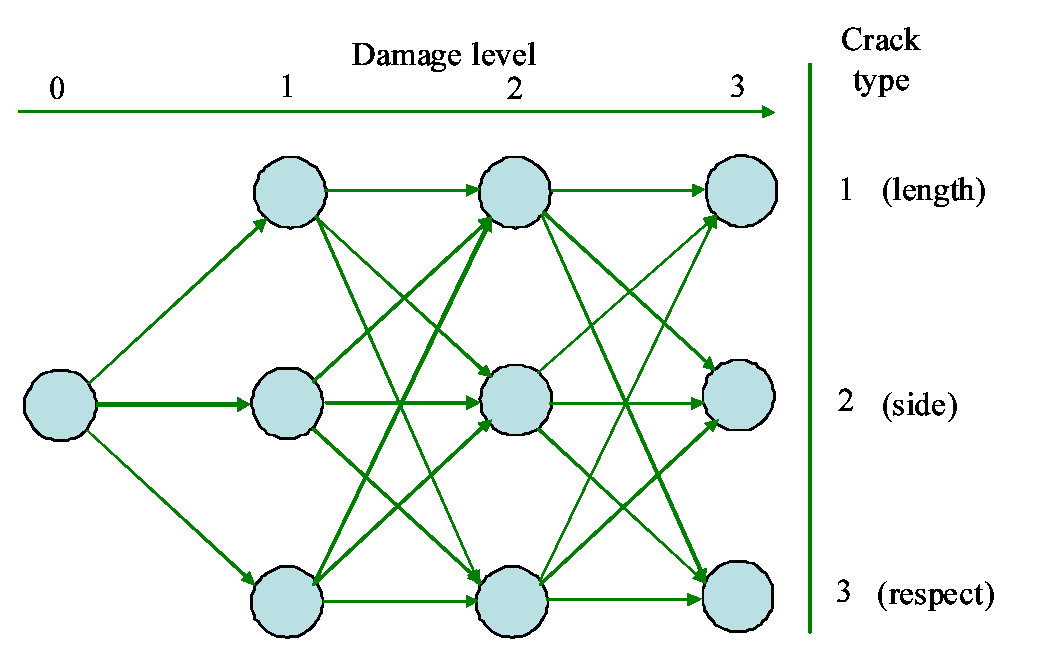
\includegraphics[scale=0.5]{fig27.eps} 
\end{center}
\footnotesize Note) $\bigcirc$ represents deterioration condition state. Deterioration is expressed as a pair ($i,j$). $i$ is referred to damage level $i(i=0,1,2,3)$ while $j$ denotes the crack type $j(j=1,2,3)$. The cracking progresses by mean of pattern transition from deterioration state $(0,0)$ to the right side of the figure.
\caption{The Process of Cracking Progress in Pavement System.}
\label{fig27} 
\end{figure}
%%%%
\begin{eqnarray}
\prod { = \left( {\begin{array}{*{20}c}
   {\pi _{00} } &  \cdots  & {\pi _{0L} }  \\
    \vdots  &  \ddots  &  \vdots   \\
   o &  \cdots  & {\pi _{LL} }  \\
\end{array}} \right)} \hspace{1mm}.\label{pi35}
\end{eqnarray}
%
where $o$ is $0$ element procession in the left low triangular of the transition matrix, $\pi_{il}(i,l=1,...,L)$ is a block procession with their components as follows:
\begin{eqnarray}
\begin{array}{l}
 \pi _{00}  = \pi _{00,00} \hspace{1mm}, \\ 
 \pi _{0l}  = (\pi _{00,l1}  \cdots \pi _{00,lR} ) \hspace{1mm},\\ 
 \pi _{il}  = \left( {\begin{array}{*{20}c}
   {\pi _{i1,l1} } &  \cdots  & {\pi _{i1,lR} }  \\
    \vdots  &  \ddots  &  \vdots   \\
   {\pi _{iR,l1} } &  \cdots  & {\pi _{iR,lR} }  \\
\end{array}} \right)\hspace{1mm}. \\ 
 \end{array}
\end{eqnarray}

We admit the fact that the property of Markov transition probability in equation (\ref{pi35}) will change its value if having any change in the duration of inspection interval. In addition, in the situation that no maintenance and repair activities have been implemented in the period between two inspections, deterioration will progress, and the transition probability will satisfy conditions $\pi_{ij,lr}=0 (i > l)$, $\sum\nolimits_{l = i}^L {\sum\nolimits_{r = 1}^R {\pi _{ij,lr} } }  = 1$:
%
\begin{eqnarray}
\begin{array}{l}
  \left. {\begin{array}{*{20}c}
   {\pi _{ij,lr}  \ge 0}  \\
   {\pi _{ij,lr}  = 0 \hspace{2mm} (when \hspace{2mm} i > l)} \\
   {\sum\nolimits_{l = i}^L {\sum\nolimits_{r = 1}^R {\pi _{ij,lr} } }  = 1}  \\
\end{array}} \right\} \hspace{1mm}.\\ 
 \end{array} \label{pt36}
\end{eqnarray}
The pair of state $(L,r)$ $(r=1,...,R)$ is understood as absorbing pair of condition states with its Markov transition probability $\pi _{Lr,Lr}$ if the condition for no maintenance and repair in the history hold.

Let us consider the transition from the pair of condition state $(i,j)$ to $(i+1,r)$. The hazard rate is the summation of transition intensity $\rho _{ijr}$ being counted in the entire domain of $r$:
\begin{eqnarray}
\theta _{ij}  = \sum\limits_{r = 1}^R {\rho _{ijr} } \hspace{1mm}.\label{tranintent}
\end{eqnarray}
 %%%%%%%%%%
\subsubsection{The Hierarchical Hazard Model Formulation}
\label{2422}
In this section, we explained the procedure to formulate the transition probability of hierarchical hazard model in the assumption that observed condition states at inspection time $t=\tau_A$, $t=\tau_B$ are $h(\tau_A)=(i,j)$ and $h(\tau_B)=(l,r)$ with inspection interval $Z=\tau_B-\tau_A$.
\begin{itemize}
\item{When $(i,j)=(l,r)$}
\end{itemize}
In this case, over the period between two inspections, there has been no sign of deterioration. The original pair of condition states $(i,j)$ remains. By a similar provision to equation (\ref{pro1}), the Markov transition probability for the pair of condition state $(i,j)$ remains in the duration $Z$ can be defined:
\begin{eqnarray}
\pi_{ij,ij}(Z)=exp(-\theta_{ij}Z)\hspace{1mm}.
\end{eqnarray}
At absorbing state ($i=L$), the probability of transition absolutely equals to 1 ($\pi_{Lj,Lj}(Z)=1$).
\begin{itemize}
\item{When $l=i+1 \leq L-1$}
\end{itemize}
In this case, the damage level changes from $\tau_A=i$ to $\tau_B=i+1$ with its transition frequency of $1$. While, the damage type (cracking form in PMS as an instance), may vary in the range of $R$ ($R$ is absorbing state for damage type). Thus, we obtain the probability density function of the transition:
\begin{eqnarray}
f_{ij} (\zeta _{ij} ) = \theta _{ij} \exp ( - \theta _{ij} \zeta _{ij} ) = \sum\limits_{r = 1}^R {\rho _{ijr} \exp ( - } \theta _{ij} \zeta _{ij} )\hspace{1mm},
\end{eqnarray}
where $\zeta_{ij}$ is the life expectancy of condition state $i$. $\rho_{ijr}$, as described earlier in equation (\ref{tranintent}), is transition intensity with respect to the change of condition state from $(i,j)$ to $(i+1,j)$. The change of condition state from $(i,j)$ to $(i+1,r)$ in the interval of inspection $[\tau_A,\tau_B)$ can  happen at any arbitrary time. In another word, it is understandable to say the deterioration may shift from time $\tau_A$ to time $s_{i+1}=\tau_A+z_{ij}, (z_{ij}\in [0,Z]$, and from that time onward till the next inspection time $\tau_B$, condition state $(i+1,r)$ remains.

Further to the change of deterioration from pair $(i,j)$ to pair $(i+1,r)$, it is obvious to say that an accurate time, at which, the change happened, can not be defined in a deterministic way. Only possible way to simulate the process is to assume the transition of condition state happens at time $(\tau_A+\bar z_{ij})\in [\tau_A,\tau_B)$. With this assumption, it is understandable that the pair of condition state $(i,j)$ remains from the inspection time $\tau_A$ until arbitrary time $\tau_A+\bar z_{ij}$ in $(i,j)$ before reaching to a new pair of condition state $(i+1,r)$. It is possible therefore to express the conditional probability density $g_{ijr}(\bar z_{ij})$, at which, happening the change of the pair of condition state from  $(i,j)$ to $(i+1,r)$ at time $\tau_A+\bar z_{ij}$:
%%%%
\begin{eqnarray}
&& g_{ijr} (\bar z_{ij} ) = \frac{{\rho _{ijr} }}{{\theta _{ij} }}\frac{{f_{ij} (z_{ij}  + \tau _A )}}{{\tilde F_{ij} (\tau _A )}} \nonumber \\ 
&& = \frac{{\rho _{ijr} \exp \{  - \theta _{ij} (\bar z_{ij}  + \tau _A \} }}{{\exp ( - \theta _{ij} \tau _A )}} = \rho _{ijr} \exp (\theta _{ij} \bar z_{ij} )\hspace{1mm}.
\end{eqnarray}
Additionally, if the entire inspection duration $Z$ is considered. The conditional probability density $q_{ijr} (\bar z_{ij})$ (at which the condition state $(i+1,r)$ remaining until inspection time $\tau_B$) can be expressible by means of the joint probability between the conditional probability $g_{ijr}(\bar z_{ij})$ and the survival probability $\tilde F_{i + 1,r} (\tau _B - \bar z_{ij} - \tau _A )$:
%%%%
\begin{eqnarray}
\begin{array}{l}
 q_{ijr} (\bar z_{ij} ) = g_{ijr} (\bar z_{ij} ) \cdot \tilde F_{i + 1,r} (\tau _B  - \bar z_{ij}  - \tau _A ) \\ 
  = \rho _{ijr} (\bar z_{ij} )\exp ( - \theta _{ij} \bar z_{ij} )\exp \{  - \theta _{i + 1,r} (Z - \bar z_{ij} )\}  \\ 
  = \rho _{ijr} (\bar z_{ij} )\exp ( - \theta _{i + 1,r} Z)\exp \{  - (\theta _{ij}  - \theta _{i + 1,r} )\bar z_{ij} \}  \hspace{1mm}.\\ 
 \end{array} \label{eq248}
\end{eqnarray}
In equation (\ref{eq248}), the elapsed time $\bar s_{i+1}=\tau_A+\bar z_{ij}$ is considered as a fixed term. However, as a matter of course, the change of pair of condition state can happen at any arbitrary time $z_{ij}$ within the inspection interval $Z$. Hence, the Markov transition probability $\pi_{ij,i+1r}$, to which, the deterioration progresses from $(i,j)$ to $(i+1,r)$ in between the two consecutive inspection times is just the integration of conditional probability $q_{ijr} (\bar z_{ij} )$ in continuous time frame:
%%% 
\begin{eqnarray}
\begin{array}{l}
 \pi _{ij,i + 1r} (Z) = {\rm{Prob}}[h(\tau _B ) = (i + 1,r)|h(\tau _A ) = (i,j)] \\ 
  = \int\limits_0^Z {q_{ijr} (z_{ij} )dz_{ij} }  = \int\limits_0^Z {\rho _{ijr} \exp ( - \theta _{i + 1r} Z)\exp \{  - (\theta _{ij}  - \theta _{i + 1r} )z_{ij} \} dz_{ij} }  \\ 
  = \frac{{\rho _{ijr} }}{{\theta _{ij}  - \theta _{i + 1r} }}\{  - \exp ( - \theta _{ij} Z) + \exp ( - \theta _{i + 1r} Z)\}  \hspace{1mm}.\\ 
 \end{array} \label{eq250}
\end{eqnarray}
In equation (\ref{eq250}), regardless of how positive or negative in the relation between $\theta_{ij}$ and $\theta_{i+1r}$ is, the value of Markov transition probability is always positive $ \pi_{ij,i+1r} > 0$.

Regarding the estimation for Markov transition probability $\pi_{ij,lr}$, a similar probabilistic inference and calculation can be derived for a general case. Details has already explained in subsection \ref{241}. The following subsection briefly describes the estimation method for useful connection.
%%%%
\subsubsection{Estimation method for hierarchical index deterioration hazard model}
\label{2423}
The obtained inspection information on sample $k$ can be described as $\bar\xi^k=(\bar \delta^k,\bar Z^k,\bar x^k)$ with the sign $\left[ {\bar {\hspace{3mm}} } \right]$ inferring an actual measurement value. $\bar \delta^k$ is an additional dummy variable receiving its value of $1$ if $h(\tau_A^k)=(i,j)$ and $h(\tau_B^k)=(l,r)$, otherwise, its value is assumed to be equal to $0$. The transition intensity $\rho_{ijr}^k (i=0,...,L-1;r=0,...,R;k=1,...,K)$, which forms a part of Markov transition probability, can be expressible through the peculiar characteristic vector $x^k$ and the unknown parameter $\beta_{ijr}$:
\begin{eqnarray}
\rho _{ijr}^k  = x^k \beta _{ijr}^{'} \hspace{1mm}.
\end{eqnarray}
Moreover, since the inspection interval $\bar Z^k$ also effects on the change of Markov transition probability $\pi_{ij,lr}$, we can express the transition probability in the functional form $\pi_{ij,lr}(\bar Z^k, \bar x^k: \beta)$. $(\bar Z^k, \bar x^k)$ is measured by inspection and $\beta=(\beta_{000},...,\beta_{L-1RR})$ is vector of unknown parameter deeming to be estimated. If assuming the mutually independence of occurrence of condition state on total $K$ samples, we are able to express the simultaneous probability density by means of log-likelihood function as follow:
%%%%%%
\begin{eqnarray}
\begin{array}{l}
 \ln \ell (\beta ) = \ln \prod\limits_{i = 0}^{L - 1} {\prod\limits_{j = 0}^R {\prod\limits_{l = i}^{L - 1} {\prod\limits_{r = 0}^R {\prod\limits_{k = 1}^K {\left\{ {\pi _{ij,lr} (\bar Z^k ,\bar x^k :\beta )} \right\}} } } } } ^{\bar \delta _{ij,lr}^k }  \\ 
  = \sum\limits_{i = 0}^{L - 1} {\sum\limits_{j = 0}^R {\sum\limits_{l = i}^{L - 1} {\sum\limits_{r = 0}^R {\sum\limits_{k = 1}^K {\bar \delta _{ij,lr}^k } } } } } \ln \left\{ {\pi _{ij,lr} (\bar Z^k ,\bar x^k :\beta )} \right\} \hspace{1mm}.\\ 
 \end{array}
\end{eqnarray}
This log-likelihood function defines that it is a function of unknown parameter $\beta$ given observational data $\bar \delta_{ij,lr}^k, \bar Z_k, \bar x^k$. Solution approach using maximum likelihood estimation to this function is similar to the approach that has already explained in section \ref{2413}.
%%%%%%%%%%%%%%%
\section{Hazard Model with Bayesian Estimation}
\label{25}
\subsection{Necessity of Bayesian estimation}
\label{251}
There are a vast number of references on Bayesian estimation worldwide. Especially, in statistic and probability area, the method in Bayesian estimation turns out to be among the powerful tool for estimation of statistical and probabilistic models under constrains of sampling population. Bayesian estimation uses the collected prior information on the behavior of event to update the probability of occurrence of event in the future \cite{wago}.

From the standpoint of infrastructure asset management, Bayesian estimation, without any doubt, indeed becomes of necessity since it is often the case that we have to estimate the model's parameters under the umbrella of small sampling data \cite{fenghong,ben-akiva93,ben-akiva95}. In addition, measurement errors and bias in observed inspection data have been reported as significant factors, which appear to violate the accuracy of estimation \cite{mishalanigong}. 
%%

Let us have a look at the \textbf{Figure \ref{fig28}} to understand the principle of powerful Bayesian estimation for infrastructure asset management. The figure illustrates three different situations when Bayesian principles are applied. Level of accuracy of hazard model will increase if plenty of prior information and observed data is available. The estimation results are thought to be improved as moving the estimation procedure on the right hand side of the Figure.

In reality, it is extremely important to apply Bayesian update rule. For examples, technology innovation in infrastructure asset would probably change the behavior of deterioration process (maintenance, repair, renovation with new technology). Thus if only relies on the past inspection without considering the changes, a wrong result may be encountered as a consequence. In another perspective, applying Bayesian estimation, we can utilize the expertise and the vast rich knowledge, which has been constantly accumulated throughout the years. As a result, we can minimize the subjective assumption in prior information.
\begin{figure}[t]
\begin{center}
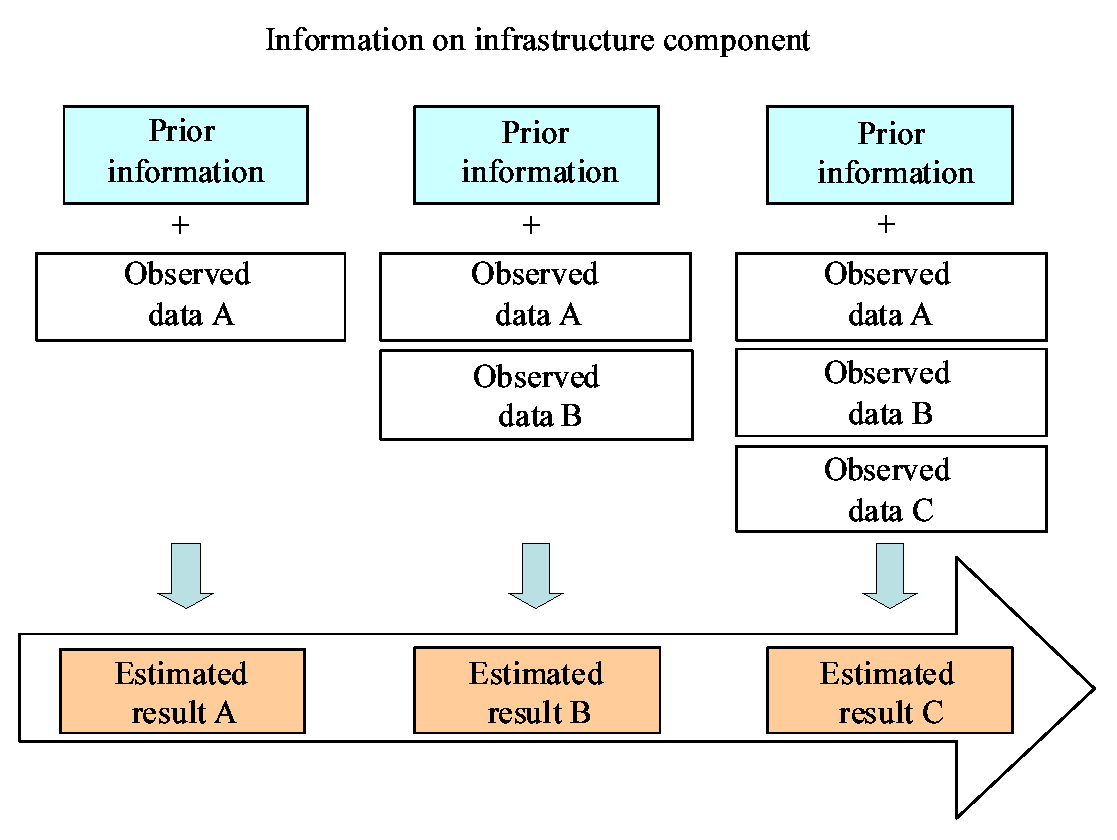
\includegraphics[scale=0.5]{fig28} 
\end{center}
\footnotesize Note) Bayesian update is applied at respective stages when having new observed data. As the sequent, accuracy level happens to increase. Moreover, the influence of prior subjective information will be weakening throughout the time.
\caption{Bayesian Update Principle Chart.}
\label{fig28} 
\end{figure}
%%%
\subsection{Bayesian estimation and its prior subjective information}
\label{252}
Maximum likelihood estimation approach, as described in section \ref{24}, is an excellent approach to estimate the model's parameter under the circumstance that numerous data has been accumulated. The reason behinds that is, as a probabilistic approach, maximum likelihood estimation illustrates the behavior of distribution of parameter around the mean. In another word, the asymptotic behavior can only be acquired if huge number of data is available. 

However, in many cases, it is hard to have a full set of sufficient data. And thus, if continuing with maximum likelihood approach, the bias in estimation results may occur, especially under data insufficiency. Furthermore, there happens a high possibility that measurement errors and bias actually exist within the sampling population. It is therefore, when Bayesian estimation is applied with use of the prior information, the estimation results can be greatly improved.

In Bayesian estimation, the posterior distribution of the parameter will be estimated by using the likelihood function defined by the employing prior distribution of parameter and observed data \cite{andrwewgel}. The likelihood function is denoted as $\iota( \left. {\theta} \right|\xi)$ with  $\theta$ and $\xi$ respectively inferring unknown parameter and observed data. Based on Bayesian theorem, the unknown parameter $\theta$ is assumed to be a random variable and the Bayesian posterior probability $\pi (\left. {\theta} \right|\xi)$ of $\theta$ given observed data $\xi$ can be defined as
%%%
\begin{eqnarray}
\pi (\left. \theta  \right|\xi ) = \frac{{\ell (\left. \theta  \right|\xi )\pi (\theta )}}{{\int_\Theta  {\ell (\left. \theta  \right|\xi )\pi (\theta )d\theta } }}, \label{bayesi}
\end{eqnarray}
where $\pi (\theta )$ is the prior probability of $\theta$ that was inferred before new evidence becoming available. The sign $\Theta$ denotes the space of unknown parameter. In some extend, it is understandable to approximate $\pi (\left. {\theta} \right|\xi)$ to the value of the nominator in equation (\ref{bayesi}):
\begin{eqnarray}
\pi (\left. \theta  \right|\xi ) \propto \ell (\left. \theta  \right|\xi )\pi (\theta ). \label{pibayesian}
\end{eqnarray}
The denominator in equation (\ref{bayesi}) is regarded as a constant term inferring the standard or the prior predicted distribution of $\pi (\left. {\theta} \right|\xi)$.:
\begin{eqnarray}
m(\xi ) = \int_\Theta  {\ell (\left. \theta  \right|\xi )\pi (\theta )d\theta }. 
\end{eqnarray}
In Bayesian updating rule, the steps of estimation are as follows: 1) Assuming the prior probability density function $\pi(\theta)$ based on the prior experience information, 2) Defining the likelihood function $\ell (\left. \theta  \right|\xi )$ based on newly observed data $\xi$, 3) Updating the probability density function $\pi (\left. {\theta} \right|\xi)$ for the parameter $\theta$ based on the Bayesian rule in equation (\ref{bayesi}). In this method, the probability distribution of unknown parameter $\theta$ is not estimated in the same way like that by using maximum likelihood estimation, but by Bayesian updating rule in the condition of obtaining the posterior distribution.
%%%%%
\subsection{Markov Chain Monte Carlo Simulation}
\label{253}
In general, there is a limitation in estimating parameter of deterioration hazard model either with maximum likelihood and Bayesian updating rule if the problem of multi-integration exists \cite{wago,titter,robert}. In recent years, Markov Chain Monte Carlo (MCMC) has been introduced in the field of Bayesian statistics, and as the sequent, greatly improve the estimation for posterior distribution without considering such a high and sophisticated level of integration \cite{wago}. 

In MCMC simulation, Gibbs sampling and Metropolis Hastings (Metropolis-Hastings or MH) techniques have been remarkably discussed \citep{wago,danihed}. Reference to image restoration was among the first application of MCMC simulation \citep{gibbs1}. Of that study, the algorithm of Gibbs Sampling was used to estimate the posterior distribution in Bayesian estimation \citep{gibbs2}. In MH law, the iterative parameter $\mbox{\boldmath$\theta$}$ is defined by repeatedly generating random numbers through the conditional probability density function $\pi (\left. {\theta} \right|\xi)$.
%%%%%%%%%%%%%
%\subsection{Bayesian estimation for Weibull deterioration hazard model}
%\label{254}
%This part presents an approach to estimate the unknown parameter $\theta$ of Weibull deterioration hazard model using the Bayesian updating rule. Reference is made to subsection \ref{234}. In this case, we assume the newly acquired data as  $\bar (\xi_1,...,\bar \xi_n)$. The likelihood function defined by Weibull distribution in equations (\ref{prop-bFlaw}) and (\ref{kikanw}) is expressed as follow
%%%%%%%%%%%
%\begin{eqnarray}
%\begin{array}{l}
% \ell (\left. \theta  \right|\bar \xi ) = \prod\limits_{i = 1}^n {f(\bar y_i ,\bar x_i :\theta )^{\bar d_i } }  \cdot \tilde F(\bar y_i ,\bar x_i :\theta )^{1 - \bar d_i }  \\ 
% =m^{\bar d} \exp \left\{ {\sum\limits_{i = 1}^n {(\bar d_i \bar x_i \beta ^{'}  + \bar d_i (m - 1)\ln \bar y_i  - \exp (\bar x_i \beta ^{'} )\bar y_i^m } )} \right\} \\ 
% \end{array} \label{ptweibull}
%\end{eqnarray}
%where $\bar d$ means the total number $\bar d = \sum\nolimits_{i = 1}^n {\bar d_i }$ corresponding to the sample, which already changed its life expectancy during the inspection period. $\theta=(m,\beta)$ is unknown parameter in Weibull hazard model. It is noted that the prior density function to likelihood function (\ref{ptweibull}) does not exist. Therefore, the function type of prior probability density function $\pi (\theta)$ and probability density function $\pi (\left. {\theta} \right|\xi)$ are multually independent in Bayesian estimation rule. 
%
%In fact, in Bayesian estimation method, the prior probability density function of parameters $m$ and $\beta$ are assumed to follow probabilistic distribution such as Gamma distribution $m \sim g(m_0 ,\kappa _0 )$ and multi-dimensional normal distribution $\beta  \sim N_k (\mu _o ,\sum\nolimits_o {} )$ respectively. The probability density function of gamma distribution $g(m_0 ,\kappa _0 ), K$ and $K$ dimensions of normal distribution $\sim N_k (\mu _o ,\sum\nolimits_o {})$ are respectively given below.
%%%%%%%
%\begin{manyeqns}
 %&& \hspace{-10mm} f(m|m_0 ,k_0 ) = \frac{1}{{\Gamma (m_0 )}}\kappa _0 ^{m_0 } m^{m_0  - 1} e^{ - \kappa _0 m}  \\ 
% && \hspace{-10mm} g(\beta |\mu o,\sum\nolimits_o {} ) = \frac{1}{{\sqrt {(2\pi )^K |\sum\nolimits_o {} |} }} 
% \exp \left\{ { - \frac{1}{2}(\beta  - \mu _o )\sum\nolimits_o^{ - 1} {(\beta  - \mu _o )^{'} } } \right\} 
%\end{manyeqns}
%where $\sum\nolimits_o$ and $\mu _o$ of $\sim N_k (\mu _o ,\sum\nolimits_o {})$ are the  covariance matrix and the standard covariance of prior distribution respectively. As a result, proportional results of probability density function $\pi (\left. {\theta} \right|\bar \xi)$ expressed in equation \ref{pibayesian} is re-formulated as follows.
%%%%%%%%%%%
%\begin{eqnarray}
%\begin{array}{l}
% \pi (\left. \theta  \right|\bar \xi ) \propto \ell (\left. \theta  \right|\bar \xi )f(m|m_0 ,k_0 )g(\beta |\mu o,\sum\nolimits_o {} ) \\ 
 % \propto m^{m_o  + \bar d - 1} \exp \left\{ {\sum\limits_{i = 1}^n {(\bar d_i \bar x_i \beta ^{'}  + \bar d_i (m - 1)\ln \bar y_i  - \exp (\bar x_i \beta ^{'} )\bar y_i^m } } \right\} - \kappa _0 m \\ 
%  - \frac{1}{2}(\beta  - \mu _o )\sum\nolimits_o^{ - 1} {(\beta  - \mu _o )^{'} }  \\ 
% \end{array} \label{pibaym}
%\end{eqnarray}
%It is assumed at this point that the value of parameter $m$ and $\beta$ are available, thus, the conditional probability density function $\pi (m|\beta, \bar \xi)$ can be defined from equation (\ref{pibaym}).
%\begin{eqnarray}
%\begin{array}{l}
 %\pi (m|\beta ,\bar \xi ) \propto m^{\hat m_o  - 1} \exp ( - \hat \kappa _0 m)\exp ( - \sum\limits_{i = 1}^n {\gamma _i \bar y_i^m } ) \\ 
 %\left\{ {\begin{array}{*{20}c}
 %  {\hat m_0  = m_0  + \sum\nolimits_{i = 1}^n {\bar d_i {\rm{      }}} }  \\
 %  {\hat \kappa _0  = \kappa _0  + \sum\nolimits_{i = 1}^n {\bar d_i \ln \bar y_i } }  \\
  % {\gamma _i  = \exp (\bar x_i \beta ^{'} ){\rm{          }}}  \\
%\end{array}} \right. \\ 
 %\end{array} \label{priorbay}
%\end{eqnarray}
%By updating rule in Bayesian estimation, the value of unknown parameter $\beta^{-j}$ in the pool of elements $\beta^{j}$  $j(j=1,...,K)$, which deems to be revealed, will be excluded from the rest of the vector $\beta$. Thus, a new estimation for $\beta^{j}$ can be realized based on conditional probability density function $\pi (\beta^{j}|m,\beta^{-j},\bar \xi)$ given already-known value of $m$ and $\beta^{-j}$.
%%%%%%%%%%%%%%
%\begin{eqnarray}
%\begin{array}{l}
 %\pi (\beta ^j |m,\beta ^{ - j} ,\bar \xi ) \propto \exp \left\{ { - \frac{{\rho _{jj} }}{2}(\beta ^j  - \hat \mu _0^j )^2 } \right\}\exp ( - \sum\limits_{i = 1}^n {\gamma _i \bar y_i^m } ) \\ 
 %\left\{ {\begin{array}{*{20}c}
 %  {\hat \mu _0^j  = \mu _0^j  + \frac{1}{{\rho _{jj} }}\left\{ {\sum\nolimits_{i = 1}^n {\bar d_i x_i^j } } \right.}  
 %  { - \left. {\sum\nolimits_{k = 1, \ne j}^K {(\beta ^k  - \mu _0^k )\rho _{kj} } } \right\}}  \\
 %  {\gamma _i  = \exp (\bar x_i \beta ^{'} ){\rm{          }}}  \\
%\end{array}} \right. \\ 
 %\end{array} \label{priorbay2}
%\end{eqnarray}
%where $\mu_0^j$ is the mean of the expected value vector $\mu_0^j$ of the multi-dimensional normal distribution $N_K(\mu_0,\sum\nolimits_0)$, which presents the prior distribution. $\rho_{kj}$ is $(k,j)$ element of retrogression row $\sum\nolimits_{0}^{-1}$ of the standard covariance and the covariance matrix. Moreover, the sum $\sum\nolimits_{k = 1,\neq j}^K$ means the total of element starting from $1$ to $K$ without considering the element $j$. The sampling algorithm can be further described in following steps.
%%%
%\begin{itemize}
%\item Step 1) Setting the initial parameter value $\theta^0=(m(0), \beta^1(0),...,\beta^K(0))$ with $i=0$ and selecting $\bar n$ samples.
%\item Step 2) Randomly generating $\theta^{i+1}=(m(i+1), \beta^1(i+1),...,\beta^K(i+1))$ in following manners.\\
%\hspace{5mm} - Randomly generating $m(i+1)$ numbers from $\pi (m|\beta(i), \bar \xi$\\
%\hspace{5mm} - Randomly generating $\beta^1(i+1)$ numbers from  $\pi (\beta^1|m(i+1), \beta^{-1}(i), \bar \xi)$\\
%\hspace{5mm} - Randomly generating $\beta^k(i+1)$ numbers from  $\pi (\beta^k|m(i+1), \beta^1(i+1), ...,$\\$ \beta^{k-1}(i+1), \beta^{k+1}(i),..., \beta^K(i), \bar \xi)$ with $(k=2, ...,K-1)$\\
%\hspace{5mm} - Randomly generating $\beta^K(i+1)$ numbers from $\pi (\beta^K|m(i+1), \beta^{-K}(i+1), \bar \xi)$
%\item Step 3) Accepting  $\theta^{i+1}$ if $i \geq n$.
%\item Step 4) Ending the calculation iteration if  $i=\bar n$. Otherwise, if $i < \bar n$, returning to $Step 2$ and increasing the level $i=i+1$.
%\end{itemize}
%In Gibbs sampling, the definition of nucleus transition $K(\theta^i, \theta^{i+1}|\bar \xi)$ is as follow
%%
%\begin{eqnarray}
%\begin{array}{l}
 %K(\theta ^i ,\theta ^{i + 1} |\bar \xi ) = \pi (m(i + 1)|\beta (i),\bar \xi )\prod\limits_{j = 1}^{K - 1} {\pi (\beta ^j (i + 1)} |m(i + 1), \\ 
 %\beta ^1 (i + 1),...,\beta ^{j - 1} (i + 1),\beta ^{j + 1} (i),...,\beta ^K (i),\bar \xi ) \cdot \\ \pi (\beta ^K (i + 1)|m(i + 1),\beta ^{ - K} (i + 1),\bar \xi ) \\ 
 %\end{array}
%\end{eqnarray}
%In this understanding, the value of $\theta^i (i=0,1,...)$ is thought to follow Markov chain with its nucleus transition $K(\theta^i, \theta^{i+1}|\bar \xi$. In addition, $\theta^i (i=n+1, n+2, ..., n)$ obtained by Gibbs sampling can be regarded as specimen sample from probability density function $\pi (\theta |\bar \xi)$, at which, satisfying the stationary state of Markov chain for a very big $n$. 
%
%After $K+1$ samples, it is possible to obtain the conditional probability density function $\pi (m|\beta, \bar \xi)$ and $\pi (\beta^j|m, \beta^{-j}, \bar \xi)(j=1,...,K)$. When the equations (\ref{priorbay}) and (\ref{priorbay2}) are considered as functions of $m$ and $\beta^j(j=1,...,K)$, then both log-likelihood functions $ln[\pi(m|\beta ,\bar \xi)]$ and $ln[\pi (\beta^j|m, \beta{-j},\bar \xi)] (j=1,...,K)$ are concave functions. It is thus, adaptive dismissal sampling becomes effectively in selecting the specimen sample from posterior distribution since having the concave shapes of probability density function. %%%%%%%%%%% 
%\subsection{Bayesian estimation for Markov hazard model}
%\label{255}
%Bayesian estimation can also be applied to estimate the unknown parameter $\beta$ of the exponential Markov deterioration hazard model, which is discussed in section \ref{241}. The rule of Bayesian estimation is carried out by using the visual inspection data of the second time. We denote $\bar \xi = (\bar \xi^1,...,\bar \xi^K)$ as the information of newly inspection data, which comprises of the information on sample $k$ as $\bar \xi^k = (\bar \delta_{ij}^k, \bar z^k, \bar x^k)$. Thus, from equation (\ref{hazardpiij}) and (\ref{logbF}), the likelihood function of exponential Markov hazard model can be re-written as
%\begin{eqnarray}
%\ell (\beta |\bar \xi ) = \prod\limits_{i = 1}^{J - 1} {\prod\limits_{j = 1}^J {\prod\limits_{k = 1}^K {\left\{ {\sum\limits_{h = i}^j {\prod\limits_{l = i}^{h - 1} {\frac{{\theta _l^k }}{{\theta _l^k  - \theta _h^k }}\prod\limits_{l = h}^{j - 1} {\frac{{\theta _l^k }}{{\theta _{l + 1}^k  - \theta _h^k }}} } } \exp ( - \theta _h^k \bar z^k )} \right\}^{\bar \delta _{ij}^k } } } } 
%\end{eqnarray}
%A standard prior probability density function of $\beta_i$ is assumed to follow multi-dimensional normal distribution $\beta_i \sim N_M(\mu_i, \sum\nolimits_{i})$. As a result, it is possible to express the probability density function $\pi (\beta|\bar \xi)$ in view of Bayesian updating rule.
%\begin{eqnarray}
%\begin{array}{l}
% \pi (\beta |\bar \xi ) \propto \ell (\beta |\bar \xi )\prod\limits_{i - 1}^{J - 1} {g(\beta |\mu _i ,\sum\nolimits_i {} )}  \\ 
 % \propto \prod\limits_{i = 1}^{J - 1} {\prod\limits_{j = 1}^J {\prod\limits_{k = 1}^K {\left\{ {\prod\limits_{l = i}^{j - 1} {\theta _l^k \sum\limits_{h = i}^j {\prod\limits_{l = i}^{h - 1} {\frac{1}{{\theta _l^k  - \theta _h^k }}\prod\limits_{l = h}^{j - 1} {\frac{1}{{\theta _{l + 1}^k  - \theta _h^k }}} } } } \exp ( - \theta _h^k \bar z^k )} \right\}^{\bar \delta _{ij}^k } } } }  \cdot  \\ 
 %\prod\limits_{i = 1}^{J - 1} {\exp \left\{ { - \frac{1}{2}(\beta _i  - \mu _i )\sum\nolimits_i^{ - 1} {(\beta _i  - \mu _i )^{'} } } \right\}} \\ 
 %\end{array} \label{markovbay}
%\end{eqnarray}
%In this sampling rule, the unknown parameter vector $\theta_{e,m}$, of which, values are excluded from $\theta$, is denoted as $\theta_{-(e,m)}$. In view of conditional probability, the probability density function $\pi (\theta_{e,m}|\theta^{-(e,m)}, \bar \xi)$ can be again expressed as follow
%\begin{eqnarray}
%\begin{array}{l}
% \pi (\beta _{e,m} |\beta ^{ - (e,m)} ,\bar \xi ) \propto \\ \prod\limits_{i = 1}^e {\prod\limits_{j = e}^J {\prod\limits_{k = 1}^K {\left\{ {\theta ^{k^{\bar \delta _{ij}^k  - \bar \delta _{ie}^k } }  \cdot \sum\limits_{h = i}^j {\prod\limits_{l = i}^{h - 1} {\frac{1}{{\theta _l^k  - \theta _h^k }}\prod\limits_{l = h}^{j - 1} {\frac{1}{{\theta _{l + 1}^k  - \theta _h^k }}\exp ( - \theta _h^k \bar z^k )} } } } \right\}} } } ^{\bar \delta _{ij}^k }  \\ 
 % \cdot \exp \left\{ { - \frac{1}{2}(\beta _e  - \mu _e )\sum\nolimits_e^{ - 1} {(\beta _e  - \mu _e )^{'} } } \right\}  
 % \propto \\ \prod\limits_{i = 1}^e {\prod\limits_{j = e}^J {\prod\limits_{k = 1}^K {\left\{ {\exp (\beta _{e,m} x_m^k )^{\bar \delta _{ij}^k  - \bar \delta _{ie}^k }  \cdot \sum\limits_{h = i}^j {\prod\limits_{l = i}^{h - 1} {\frac{1}{{\theta _l^k  - \theta _h^k }}\prod\limits_{l = h}^{j - 1} {\frac{1}{{\theta _{l + 1}^k  - \theta _h^k }}\exp ( - \theta _h^k \bar z^k )} } } } \right\}^{\bar \delta _{ij}^k } } } }  \\ 
 % \cdot \exp \left\{ { - \frac{{\rho _e^{mm} }}{2}(\beta _{e,m}  - \hat \mu _e^m )^2 } \right\} \\ 
% \hat \mu _e^m  = \mu _e^m  + \sum\limits_{h = 1, \ne m}^M {(\beta _{e,h}  - \mu _e^h )} \rho _e^{mm}  \\ 
% \end{array}
%\end{eqnarray}
%In this conditional probability density function, value of $\beta_{e,m}$ is thought to conditionally depend on $\beta^{-(e,m)}$, which has already revealed from equation (\ref{markovbay}). $\delta_{ie}^k$ is the dummy variables receiving its value of $1$ when prior rating $e$ is obtained from Gibbs sampling with prior rating $d(\tau_A^k)=i$ on the sample $k$, otherwise value of the dummy variable equals to $0$. $\mu_e^m$ is the median of the prior expected value vector $\mu_e$. $\rho_e^{hm}$ is $(h,m)$ element of the prior standard covariance of procession $\sum\nolimits_{e}^{-1}$. In addition, $\sum\nolimits_{h=1,\neq m}^{M}$ is the sum of total elements counting from $1$ to $K$, excluding element $m$. The specimen is randomly generated from conditional probability density functions. And thus, the generated specimen can be used to infer the posterior distribution of the unknown parameter $\beta$. 
%%%%
%\section{Hazard model and measurement errors}
%\label{26}
%\subsection{Sample loss and measurement errors}
%\label{261}
%Actual application of deterioration hazard model requires data from monitoring. For instance with Markov model, at least two set of inspection data in two different time series are needed to configure the matrix of Markov transition probability. Thus, the accuracy of estimation depends largely on how accurate level of data gathered from inspection is. If measurement errors or bias exist in the measurement, result from estimation has tendency to differ from what actually progress in the reality. Measurement errors and bias can possibly occur due to mistakes of either inspectors or monitoring equipments as well as bias assumption of condition states. Thus, the problem of measurement errors occurring in hazard model due to bias data shall be well addressed.

%Condition state of infrastructure system is often evaluated by use of average or weighted values from various indexes measured by monitoring and inspection activities. For example, in pavement management system (PMS), the Pavement Condition Index  (PCI)\footnote{PCI is a standard performance indicator, which is widely applied in the America. Other similar performance indictors have also applied in other developed countries. For example, MCI (Maintenance Control Index) is used in the PMS of Japan. The definition of PCI or MCI is largely depending on management perspective of each country.} is the weighted value of cracking, international roughness index (IRI), flatness, etc \citep{shahin05}. However, because of the measurement errors, true condition state may not be captured. Let us have a look in to the description of Figure \ref{fig29}, as an example in PMS, for better understanding of the issue.
%\begin{figure}[t]
%\begin{center}
%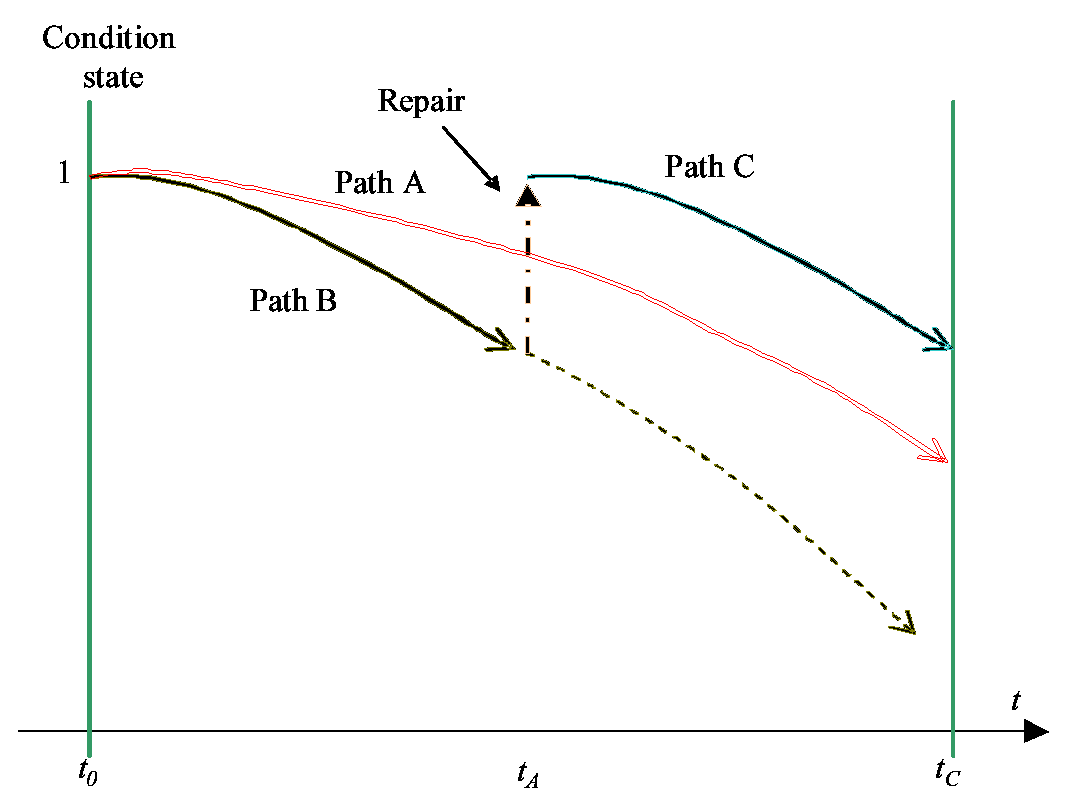
\includegraphics[scale=0.5]{fig29} 
%\end{center}
%\caption{Sample loss and measurement error due to repair}
%\label{fig29} 
%\end{figure}
%
%It is assumed in the figure that at time $\tau_0$, repair is carried out to renew the condition state of pavement to level $1$. If no other repair is carried throughout the period from $\tau_0$ to $\tau_C$, the deterioration curve is likely to follow Path A. In fact, the deterioration progress actually get worsen, and thus, the deterioration progresses like in Path B. In this condition, at time $\tau_A$, repair is imposed and deterioration curve becomes Path C. As the matter of course, if no repair is implemented at $\tau_A$, the deterioration curve will be illustrated in dotted line. However, from the monitoring and measurement standpoint, we only have information at inspection time $\tau_C$. Whereas, the information on repair has not been properly recorded. This type of problem negatively results in inaccurate estimation results of the hazard model.
%
%\begin{figure}[t]
%\begin{center}
%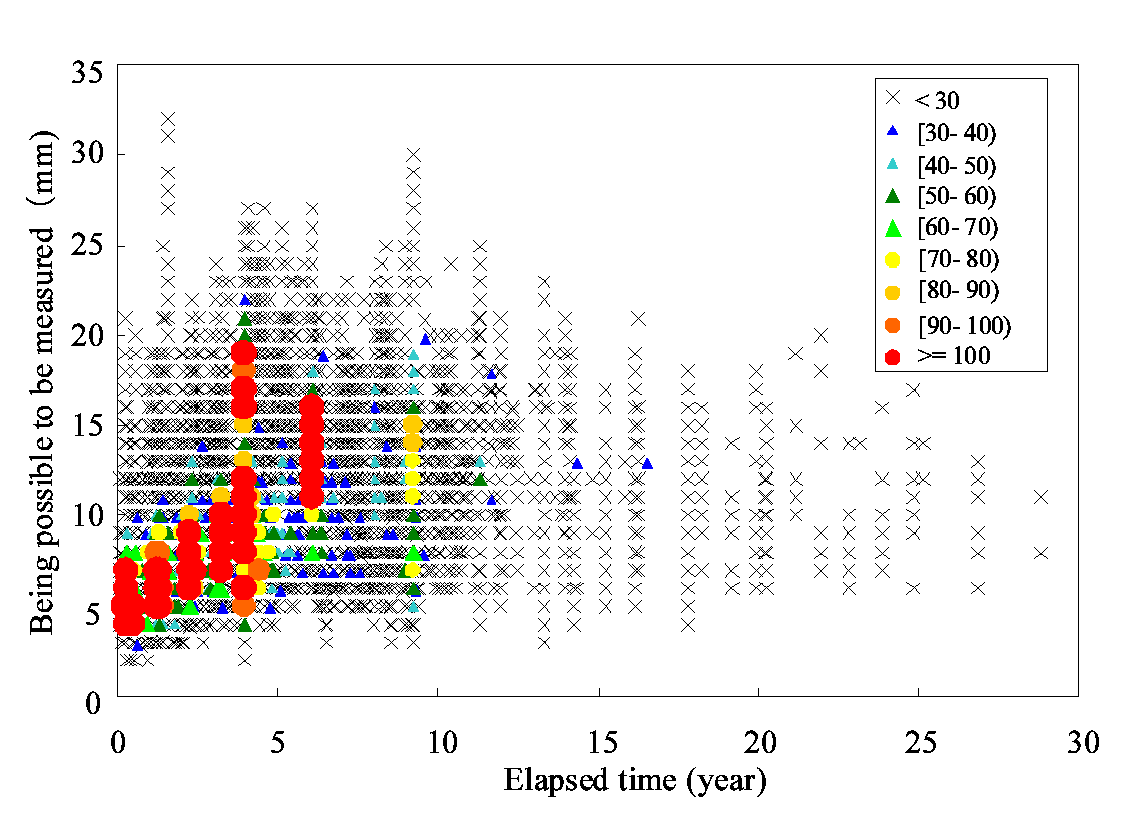
\includegraphics[scale=0.5]{fig210} 
%\end{center}
%\caption{Distribution of measurement sample-rut index (mm)}
%\label{fig210} 
%\end{figure}
%Figure \ref{fig210}, on another perspective, illustrates the problem of measurement errors. The horizontal axis shows the elapsed years, while the vertical axis expresses the possibility of capturing the rut index of road. In the period of 6 years from the opening of the road, there is an abundant amount of samples being recorded. However, the numbers of sample are slowly decrease along with time. Consequently, loss of sample happen. In reality, the condition states are largely distributed with respect to the elapsed time. A deterministic relation of this distribution may not easy to be figure out. In order to overcome this obstacle, following section further highlights the correcting methodology applying on exponential Markov hazard model in case of measurement errors and sample loss.
%%%%%%%%%%%%%
%\subsection{Maximum likelihood estimation method with sample loss}
%\label{262}
%This subsection presents the estimation method for multi-state exponential hazard model in the case of having sample loss. Particularly, dicussion is in close link to the case of pavement management system. However, as a matter of fact, the methodology can be generalize to other infrastructure types.
%
%Let us continue to drawn the case, to which, observations are conducted on sample $k(k=1,...,K)$ at two respective times $\tau_A^k$ and $\tau_B=\tau_A^k+z^k$ with $z^k$ as inspection interval. The condition state being observed at at $\tau_A^k$ and $\tau_B$ are $h(\tau_A^k)=i^k$ and $h(\tau_B^k)=j^k$ respectively. It is assumed at this state that the mentioned condition states being observed in the period $[\tau_A^k, \tau_B^k]$ are prior condition states of the road sections. Addition to the condition states, the information on characteristic variables $x^k=(x_1^k,...,x_M^k)$ are also available as results of inspections. And moreover, it is acknoledged that condition states and concerning characteristic variables are absolutely recorded for all road sections in the total $K$ sections. In short, inspection information of sample $k$ can be expressible by vector $\bar \xi^k=(\bar h(\tau_A^k),\bar h(\tau_B^k), \bar z^k, \bar x^k)(k=1,...,K)$ with [$\bar{\hspace{2mm}}$] referring to the measureable value.
 %
%In reality, inspection activities are scheduled during the management term. The time of inspection is denoted as $z_n (n=1,...,N)$. The actual numbers of characteristic varialbes being revealed through inspections are $x_l (l=1,...,L)$. Based on the obtained inspection information, it is possible to estimate the so-called ``relative frequency'' $\mu(i,z_n,x_l)$ or relative distribution of sample with its atrribute $(i,z_n,x_l)(i=1,...,J-1;n=1,...,N;l=1,...,L)$. Saying in another words, the relative distribution coefficient is deem as known parameter, which is easily obtained from data. On the other hand, the probability (or likelihood) for the simultaneous occurence of the extracted sample, being with its attribute $(i,j,z_n,x_l)$, can be presumed as likelihood function $f(i,j,z_n,x_l:\beta)$ with unknown paramater $\beta$.
%
%In statistic view, sample loss mechanism is considered to be under the shadow of probabilistic manner, and thus, the sample loss can be defined by the rate of sample loss. The loss of sample generally happens when information concerning early maintenance and repair actions on the road section prior to the next inspection time is not recorded. In fact, maintenance and repair actions are carried out on the road sections exerting with faster deteriorations than predictions. If no M\&R has yet been imposed, the prior initial condition state $i$ will deteriorate into condition state $j$. 
%
%n this situation, we express a set of sample with its pair of condition states $(i,j)(i<j)$ by $\Omega$. The possible number of sub-set $\Omega_{ij}(j=i,...,J;i=1,...,J-1)$ is $(J-1)(J+2)/2$. Another way to express the sample set is throught the union $\Omega=\cap_{i=1}^{J-1}\cap_{j=i}^{J} \Omega_{ij}$ with its empty set denoting as  $\Omega_{ij}\cap\Omega_{i^{'}j^{'}}=\phi((ij)\neq(i^{'}j^{'}))$. As a matter of course, based on the information on observed condition states, it is clear to determine the subset, to which, the sample being considered actually belongs to. Furthermore, we can exclude the sample concerning the road section with implemented M\&R during inspection interval. This sample does not belong to any proper subset of sample, and thus, it can be regarded as a sample loss.
%
%Regarding each sample subset $\Omega_{ij}$, it is understanable to define the conditional probability $Q(z_n,x_l|i,j)$ of simultaneous occurence with respect to inspection time and characteristic variables $(z_n,x_l)$. Such a simultaneous occurence probability is concretly defined for each subset of sample. In another words, the sample mechanism generation is different in each sample subset. 
%
%It is acknowledged that among samples obtained by measurement, there are $N_{ij}$ samples belong to sample subset $\Omega_{ij}$. To express the measurement sample, which is randomly extracted from $N_{ij}$ of the sample subset $\Omega_{ij}$, we use the vector $\xi = (\xi^1,...,\xi^{\bar K})$, where $\sum\nolimits_{i=1}^{J-1}\sum\nolimits_{j=1}^{J}N_{ij}=\bar K$. Due to the existence of sample loss, the sum of $N_{ij}$, which is corresponding to numbers $\bar K$ of samples, only indicate to the road sections without any M\&R during the inspection interval. Further to this matter, it is also strongly noted that the rate concerning the sample extraction is different in each samplem subset. 
%
%Theoritically, if there have been no M\&R, the condition state distribution of road section at time $\tau_B$ shall change depending on the prior condition state $i$ measured at inspection time $\tau_A$. In another words, it is possible to express the dependence distribution by describing it as conditional probability density function $\tilde P(j|i,z_n,x_l:\beta)=\pi_{ij}(z_n,x_l:\beta)$, which concerns the distribution of condition state $j$ depending on prior condition state $i$, the inspection interval $z_n$ and the characteristic variable $x_l$. As the sequent, the dependence distribution of condition state at inspection time $\tau_B=\tau_A+z_n$ can be expressed by means of conditional probability density function $P(j|i,z_n,x_l:\beta)=\pi_{ij}(z_n,x_l:\beta)$ and the distribution $\nu(z_n,x_l|i)$ of prior condition state $i$.
%%%
%\begin{eqnarray}
%\begin{array}{l}
 %\tilde Q(j|i:\beta ) = \sum\limits_{n = 1}^N {\sum\limits_{l = 1}^L {\tilde P(j|i,z_n ,x_l :\beta )\nu (z_n ,x_l |i)} }  \\ 
% (i = 1,...,J - 1;j = 1,...,J) \\ \label{pt57}
 %\end{array}
%\end{eqnarray}
%%%
%With reference to the earlier paragraph of this subsection, we can define the simultaneous probability $f(i,j,z_n,x_l:\beta)$ as follows.
%%%%%%%%%%%%%
%\begin{eqnarray}
%&& f(i,j,z_n ,x_l :\beta ) = \nonumber \\
%&& \tilde Q(j|i:\beta )Q(z_n ,x_l |i,j:\beta )\mu (i) = P(j|i,z_n ,x_l :\beta )\mu (i,z_n ,x_l ) \label{pt58}
%\end{eqnarray}
%%%%%%%%%%
%Equation \ref{pt58} can be further expressed in following equation.
%%%
%\begin{eqnarray}
%Q(z_n ,x_l |i,j:\beta ) = \frac{{P(j|i,z_n ,x_l :\beta )\mu (i,z_n ,x_l )}}{{\tilde Q(j|i:\beta )\mu (i)}} \label{pt59}
%\end{eqnarray}
%%
%The simultaneous probability $Q(z_n,x_l|i,j:\beta)$ expressed in equation \ref{pt59} reflects the conditional probability that the measurement sample concerning $(i,j,z_n,x_l)$ is randomly extracted from the sample subset $\Omega_{ij}$. By employing the definition in equation \ref{pt59}, the problems of sample loss, measurement errors and bias can be eliminated. To further describe the behavior of distribution $\nu(z_n,x_l|i)$ in equation \ref{pt57}, let express the distribution weight $w_{n,l|i}$ concerning the prior condition state $i$ with respect to inspection interval $z_n$ and characteristic variable $x_l$ in the following equation. 
%%%
%\begin{eqnarray}
%w_{n,l|i}  = \frac{{ \# \{ k \in \Omega _i |i^k  = i,z^k  = z_n \hspace{2mm} and \hspace{2mm}  x^k  = x_l \} }}{{ \ne \{ k \in \Omega i|i^k  = i\} }}
%\end{eqnarray}
%
%where $\# \lbrace k|B \rbrace$ describes the number of samples, to which, condition $B$ is satisfied. In another view, it is understood that the sample with attributes $(i^k,z^k,x^k)$ shall be neglected by filtering from the set $\Omega_i=\cup_{j=i}^J\Omega_{ij}$. Thus, theoretically, the condition state distribution $\tilde Q(j|i:\beta)$ can be further defined as follow.
%%
%\begin{eqnarray}
%\tilde Q(j|i:\beta ) = \sum\limits_{n = 1}^N {\sum\limits_{l = 1}^L {w_{n,l|i} \pi _{ij} } } (\bar z_n ,\bar x_l :\beta )
%\end{eqnarray}
%%
%Asking for the measurement sample $\bar \xi =(\bar \xi_1,...,\bar \xi_{\bar K})$, which is randomly extracting from the sample subset $\Omega_{ij}$ based on equation \ref{pt59}, the likelihood functions corresponding to the sample loss or bias elimination can be consequently defined.
% 
%\begin{eqnarray}
%\ln \tilde \ell (\bar \xi ,\beta ) = \sum\limits_{i = 1}^{J - 1} {\sum\limits_{j = i}^J {\left\{ {\sum\limits_{k = 1}^{\bar K} {\bar \delta _{ij}^k \ln \pi _{ij} (\bar z^k ,\bar x^k :\beta ) - N_{ij} \ln \tilde Q(j|i:\beta )} } \right\}} } \label{pt62}
%\end{eqnarray}
%where, as previously mentioned, $N_{ij}$ is the number of measurement samples belonging to sample subset $\Omega_{ij}$. $\bar \delta_{ij}^k$ is a dummy variable, which receives its value of $1$ when condition ($\bar h(\tau_A^k)=\bar i$ and $\bar h(\tau_B^k)=\bar j$) statisfy, otherwise, its value is assumed to equal to $0$. To this points, we can use several numerical method like maximum likelihood estimation to solve the equation \ref{pt62} in order to estimate the expected values of models's parameters.
%%%
\section{Example of Empirical Application to Infrastructure Asset Management}
\label{27}
This section discusses the possibility of applying the hazard model on infrastructure asset management at strategic level. Details of estimation is referred to paper of \citet{aokia}. In his paper, Weibull hazard model is employed to suggest the optimal timing of inspection and figure out the best possible renewal policies on tunnel lighting system, which composes as an important structure of expressway. The study focused on deriving the Markov chain process along with Weibull distribution, and further combined hazard model with life cycle cost analysis based on the existing list of renewal.

This model enables to evaluate for not only renewal cost of an individual lighting lamp (low-pressure sodium lamp) but also its optimal inspection time and the cycle of compulsory renewal. Further more, as a general requirement of management; an amount of necessary fixed cost is also generated based on least life cycle cost estimation. The model can also be extended to incorporate various types of risks in form of economic term like loss of money due to traffic congestion, which results from either incident of lighting lamp or inspection and renewal activities. As the sequent, the problem concerning the trade-off situation for inspection period, fixed cost, renewal cost can be successfully tacked. Thus, administrators can save the budget and effectively manage the system in the end.

As can be seen from Figure \ref{fig211}, administrators are able to predict the probability of survival in general for the entire lighting system. This survival probability (vertical axis) decreases along the operation time (horizontal axis) is estimated by use of equation (\ref{hazardw}) in section \ref{234}. By categorizing the lighting system into several types, it is also possible to compare the deterioration curves among those types. This kind of survival probabilities, deterioration curves, estimated by Weibull hazard model eventually turn out to be the input of life cycle cost evaluation, which is further displayed in Figure \ref{fig212}.
\begin{figure}[t]
\begin{center}
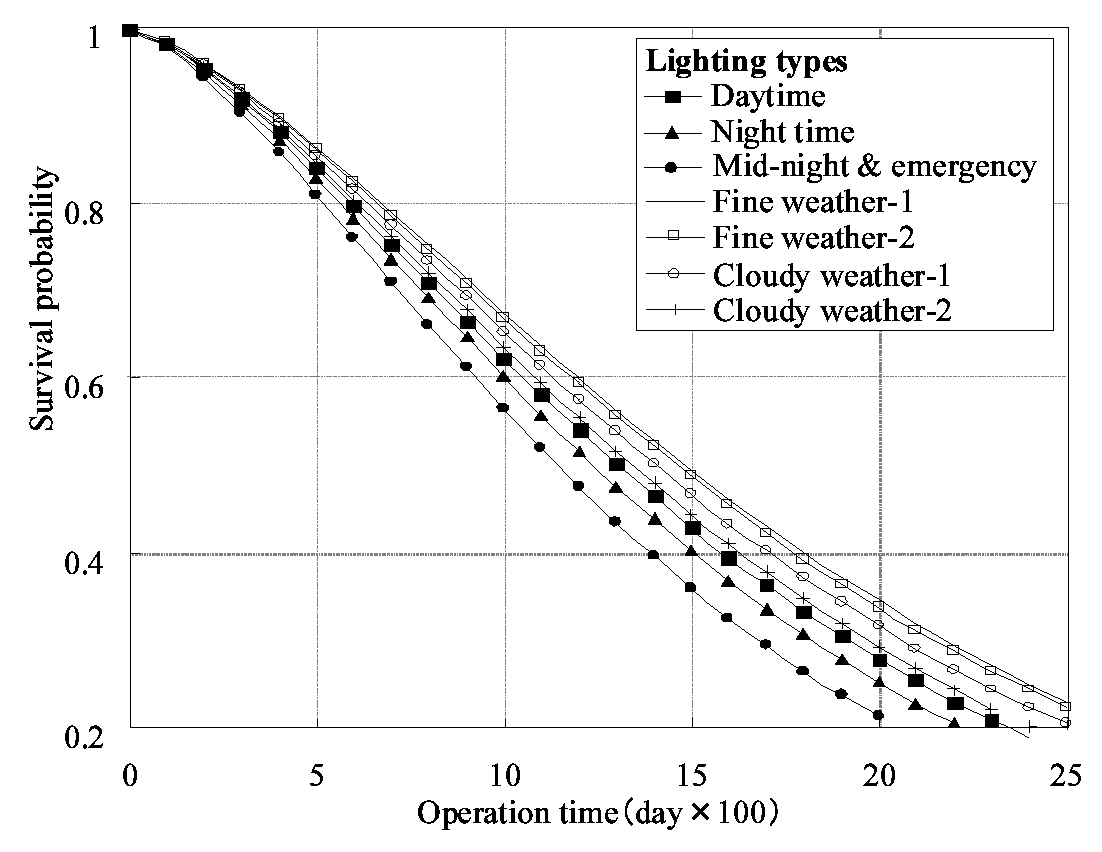
\includegraphics[scale=0.5]{fig211} 
\end{center}
\caption{Survival Probability of Tunnel Lighting Lamp (low-pressure sodium lamp).}
\label{fig211} 
\end{figure}
%%
\begin{figure}[t]
\begin{center}
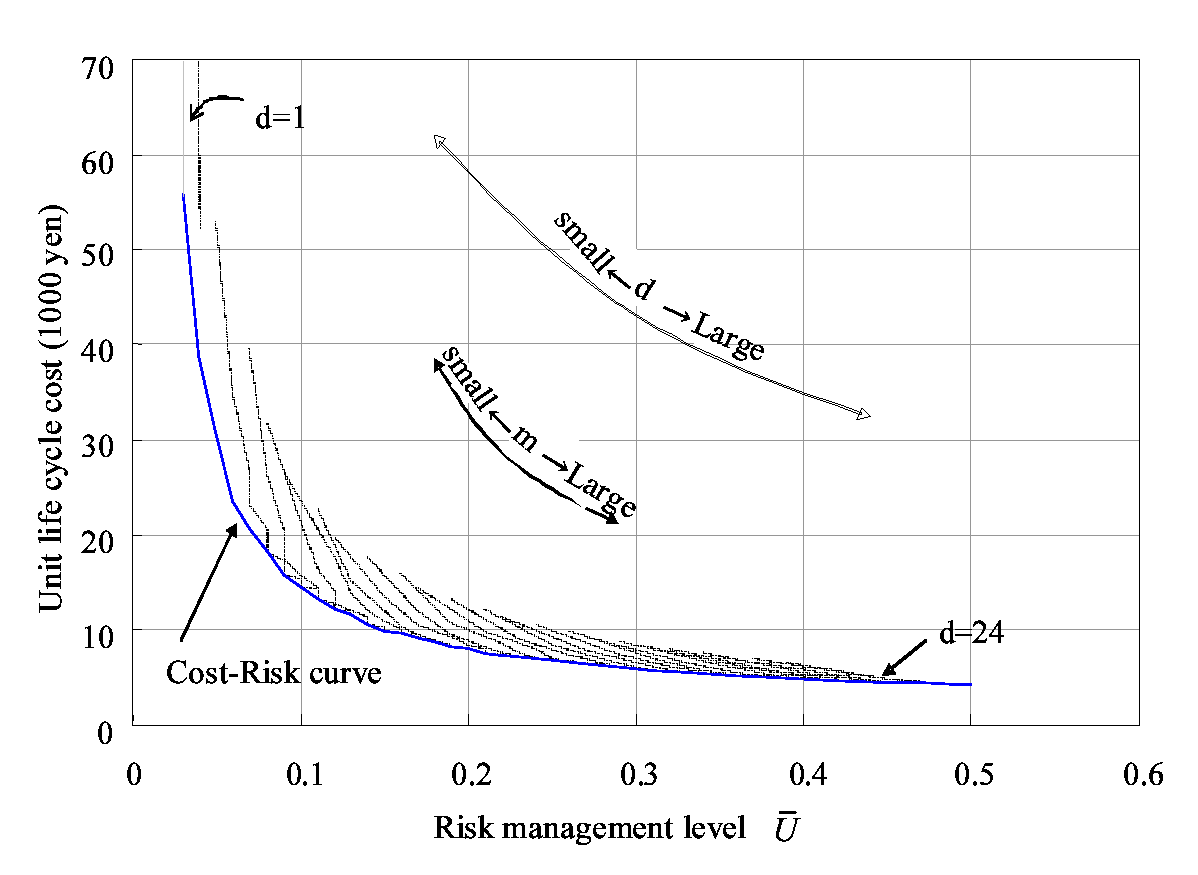
\includegraphics[scale=0.5]{fig212} 
\end{center}
\footnotesize Note) Curve is drawn based on $N=100$ lamps, at the risk management level of 0.05, the C-U curve is showed in dotted line. The solid line explains the C-U relation, which belong to possible management objective.
\caption{Cost-Risk Curve.}
\label{fig212} 
\end{figure}

Figure \ref{fig212} expresses the relation between life cycle cost of tunnel lighting system and the risk management level by drawing the cost-risk curve. The life cycle cost is a summation of inspection cost, inspection cost, renewal cost (if applied) and traffic restriction cost. Whilst, the risk management level is in fact concerning the elapsed time in operation of lighting lamp counting from beginning to the time, at which, encountering the breakdown. In another work, it concerns the so-called Value at Risk (VaR). As can be seen from Figure \ref{fig212}, the relation between trade-off is, as the risk management level grows on the right side of the horizontal axis, then the life cycle cost becomes smaller. In another meaning, the length of inspection interval sketches longer and maximum operation time of lighting lamp is determined. In contrast, as the risk management level becomes smaller than 0.1, the life cycle turns to get an intense upturn. It might be a save option to select the risk management point from 0.2 onward because the variation in change of life cycle cost is in a small scale.
%%%%%%%%%%
\section{Summary and Recommendations}
\label{28}
This chapter has presented a profound literature review on the hazard analysis in infrastructure management system. It strongly emphasized the importance of infrastructure management system in today modern society with its central role, which aims to provide the best service for society systematically. Attention has been given to analytical approach and model formulation based on stochastic methodology. Moreover, the importance role of monitoring and a good inventory box in the system has also been realized throughout the texts. Markov chain model has received a special attention, it possibly become one of a central model for any further extension.

In addition, this chapter has strongly emphasized the application of Bayesian estimation method and Markov Chain Monte Carlo (MCMC) simulation technique. Bayesian estimation combined with MCMC simulation becomes a powerful approach to tackle the issues of limited monitoring sampling data, measurement errors, bias and loss of sample. This would become a very promising horizon for future researches. Moreover, this section has briefly discussed the combination of hazard model and life cycle cost analysis, which is, without any doubt, compulsorily required in any infrastructure management system.

Based on the theory and model discussed in this chapter, the writings and discussion in subsequent chapters of this dissertation will further explore our mathematical formulation of hazard models with empirical studies on selected infrastructure networks such as tunnel lighting system, pavement system and pipeline system.
%%%%%%%%%%%%%%%%
% This is the end of chapter 2 (literature review)
%%%%%%%%%%%%%%%%%

